% Chapter 2

\chapter{Tools for Functional Data Analysis}\label{chap2} % Main chapter title

\label{Chapter2} % Change X to a consecutive number; for referencing this chapter elsewhere, use \ref{ChapterX}

\lhead{Chapter 2. \emph{Tools for Functional Data Analysis}} % Change X to a consecutive number; this is for the header on each page - perhaps a shortened title

%--------------------------------------------------------------------------------------
%	SECTION 1
%--------------------------------------------------------------------------------------

This chapter will serve to familiarize the reader with the different tools throughout this dissertation to analyse of Functional Data. The emphasis will be on the relevant techniques and methods that are applied throughout this dissertation. Some examples of fitting basis functions will be performed with their respective plots to bring clarity in the transformation of discretized observed data to functional data. A deeper look into the  Mathematics of Functional Data Analysis will be covered in the following chapter \textit{Mathematics of Functional Data Analysis}.\\
This chapter is organized as follows: \textbf{section 2.2} introduces the functional basis expansion techniques; \textbf{section 2.3} focuses on model estimation;  \textbf{section 2.4} introduces the different types of model criteria (\textit{Generalized Cross-Validation}, \textit{Generalized Information Criteria}, \textit{modified Akaike Information Criteria} and \textit{Generalized Bayesian Information Criteria}); \textbf{section 2.5} defines descriptive statistics in Functional Data framework; \textbf{section 2.6} introduces parallel computing using \texttt{R} and \textbf{section 2.7} explains how to use the University of Cape Town high performance computing facilities.


\section{Introduction}\label{intro}

In the Functional Data Analysis context, observed data are regarded as depicting an underlying function at various locations; hence each curve is treated as a single functional entity. Smoothing the Functional Data has a primary role in FDA, as it provides insight in the functional behaviour of the stochastic process.\\
For any data analysis in the FDA context, the very first step is to derive smooth Functional Data; smoothness in the sense of possessing a certain number of derivatives. Let $t$ be a one-dimensional argument sometimes referred as time. Functions of $t$ are observed over a discrete grid $\left\lbrace t_{1},\dots,t_{J} \right\rbrace \in \mathcal{T}$ at sampling values $t_j$, which may or may not be equally spaced. In order to create a functional \textit{datum}, a basis needs to be specified. The chosen basis is a linear combination of functions defining the functional object. A functional observation $X_i$ is defined as follows:
\begin{equation}\label{fda_21}
X_i(t) \approx \sum_{k=1}^{K} c_{ik}\phi_{k}(t),\text{ }\forall t \in \mathcal{T}
\end{equation}
where $\phi_{k}(t)$ (for $k = 1,\dots,K$) is the $k^{th}$ basis function of the expansion and $c_{ik}$ is the corresponding coefficient. Generally, the observerd data are filled with observational errors (or noise) that are superimposed on the underlying signal. In the real world, a typical scenario involves $N$ processes beign observed at the same time. Let $\mathbf{Y}$ be a vector of $N$ Functional Data $\bm{Y} = \left[\bm{Y}^T_{1},\dots,\bm{Y}^T_{N}\right]^T$, where each Functional Data are written as follows:
\begin{equation}\label{fda_22}
Y_{ij} = X_{i}(t_{j}) + \epsilon_{ij},\text{ } 1 \leq j \leq J \text{, } 1 \leq i \leq N.
\end{equation}
$Y_{ij}$ is a noisy observation of the stochastic process $X_{i}(t_j)$ and $\epsilon_{ij}$ is a random error with zero mean and variance function $\sigma^{2}_i$ associated with the $i^{th}$ functional datum. \\
As an illustration consider the \texttt{Aemet} dataset from the \texttt{R}-package \texttt{fda.usc} \citep{fda.usc}. It contains daily measurements of Temperature, Wind Speed and Precipitation from $N = 73$ different weather stations in Spain from 1980 to 2009. In this context, a functional observation consists of 365 pairs $(t_{j},Y_{ij})$ with $t_{1} = 0.5,\dots,t_{365} = 364.5$ ($J = 365$). Figure \ref{fig:FDA1} shows a plot of the raw data for the stations in \texttt{Alicante} and in \texttt{Oviedo}.
\begin{figure}[h]
  \centering
    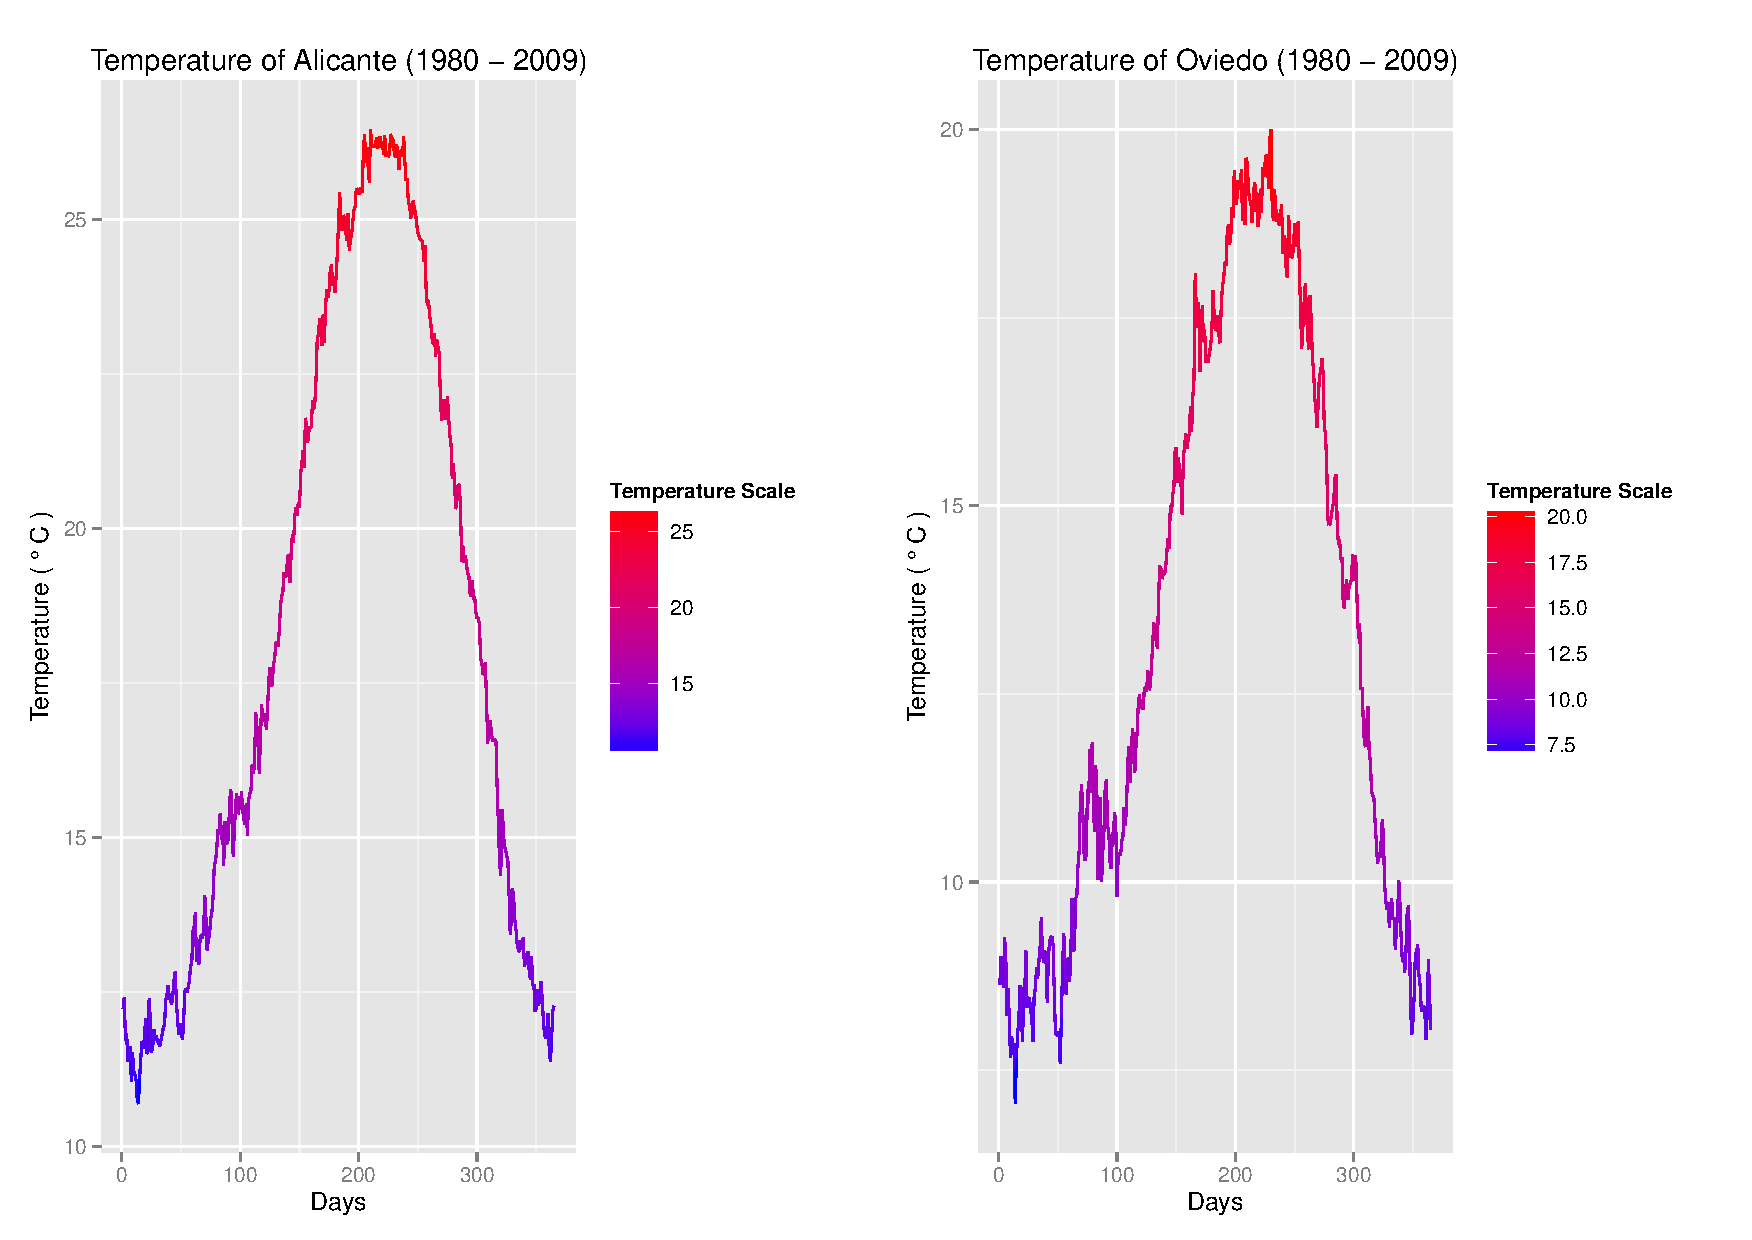
\includegraphics[width=1.1\textwidth]{Figures/temp_plot.pdf}
%    \rule{35em}{0.5pt}
  \caption[Temperature data from \texttt{Alicante} \& \texttt{Oviedo}]{Temperature data from \texttt{Alicante} \& \texttt{Oviedo} stations in Spain (1980 - 2009)}
  \label{fig:FDA1}
\end{figure} 
 In regression problems, it is very likely that the true function $X(t) = \mathbb{E}(Y|t \in \mathcal{T})$ is a nonlinear function of $t$. Representing $X(t)$ by a linear model is usually appropriate, and sometimes a necessary approximation. It is convenient because a linear model is easy to interpret and is the first-order Taylor approximation to $X(t)$ \citep*{hastie_09_elements-of.statistical-learning}. In practice, it is impossible to observe the functional values in continuous time. Smoothing methods using basis expansions are used to trim the erratic pattern of the stochastic process. They provide a good approximation to Functional Data given that the basis functions have the same essential characteristics as the process generating the data, hence minimizing the noise in raw data for calculations and analysis.\\ 
There are several types of basis expansions that can be applied to Functional Data.
\clearpage
%---------------------------------------------------------------------------------------
%	SECTION 2
%---------------------------------------------------------------------------------------

\section{Smoothing Techniques using Basis Expansion}\label{basis_expansion}

As stated in the previous section, the first step in FDA is to reconstruct the functional form of the sample curves from their discrete observations. The sample curves are assumed to be observations of a stochastic process $X = \left\lbrace X(t):t \in \mathcal{T} \right\rbrace$ whose sample functions belong to the Hilbert space $L^{2}(T)$ of square integrable functions with the inner product $\langle X_{1},X_{2} \rangle_{L_{2}} = \int\limits_{\mathcal{T}}X_{1}(t)X_{2}(t)dt,\text{ } \forall X_{1},X_{2} \in L^{2}(\mathcal{T})$. From the previous section, we have seen that any stochastic process can be approximated by taking a weighted sum or \textit{linear combination} of a sufficiently large number \textit{K}. Equation \eqref{fda_21} is written as follows:

\begin{equation}\label{fda_23}
   X_{i}(t) \approx \mathbf{c}^{T}_{i}\boldsymbol\phi(t),\text{ }\forall t \in \mathcal{T},\text{ } i = 1,\dots,N
\end{equation}

where $\mathbf{c}_{i} = \begin{bmatrix}
c_{i1}\\
c_{i2}\\
\vdots\\
c_{iK}
\end{bmatrix}$ and $\bm{\phi}(t) = \begin{bmatrix}
\phi_{1}(t)\\
\phi_{2}(t)\\
\vdots\\
\phi_{K}(t)
\end{bmatrix}$. Equation \eqref{fda_23} can be written in matrix notation as:
\begin{equation}\label{fda_24}
   X_i(\bm{t}_i) \approx \bm{\Phi}(\bm{t}_i) \mathbf{c}_i,\text{ }\forall t \in \mathcal{T}.
\end{equation}

where $\mathbf{\Phi}(\bm{t}_i)=\begin{pmatrix}
\phi_{1}(t_{i1}) & \dots & \phi_{K}(t_{i1})\\
\vdots & \ddots & \vdots\\
\phi_{1}(t_{i1}) & \dots & \phi_{K}(t_{iJ})
\end{pmatrix}$ is a $J \times K$ matrix of basis functions evaluated at each time point $t_j$.\\
Basis functions expansion represent the potentially infinite-dimensional universe of functions within the finite-dimensional framework of vectors like $\mathbf{c}$ \citep{olberd:ramsay}. A great deal depends on how the vector of basis functions $\bm{\phi}(t)$ is chosen.
\clearpage

\subsection{Fourier Basis}
The most appropriate basis for periodic functions defined on an interval $\mathcal{T}$ is the \textit{Fourier Basis} where the $\phi_{k}$'s take the following form:
\begin{equation}\label{fouriereq}
   \phi_{o}(t) = 1/\sqrt{|\mathcal{T}|},\; \phi_{2r-1}(t) = \dfrac{sin(r\omega t)}{\sqrt{|\mathcal{T}|/2}} \; \text{and} \; \phi_{2r}(t) = \dfrac{cos(r\omega t)}{\sqrt{|\mathcal{T}|/2}}
\end{equation}
for $r=1,\dots,\frac{K-1}{2}$, where $K$ is the number of basis functions; notice that the $K$ must be an odd number to compute \textit{Fourier Basis}. The frequency $\omega$ determines the period and the length of the interval $|\mathcal{T}|=2\pi/\omega$. The function vector $\bm{\phi}(t)$ has the form $\bm{\phi}(t) = \left[\phi_{0}(t),\phi_{1}(t),\phi_{2}(t),\dots,\phi_{2r}(t)\right]^T$ evaluated at discrete time points $t_{j}, \text{ }j=1,\dots,J$.\\
The \textit{Fourier Basis} defined above is said to be orthogonal if the values of $t_{j}$ are equally spaced on $J$ and the period is equal to the length of $\mathcal{T}$. Because of the orthogonal property, the cross-product $\mathbf{\Phi^{T}\Phi}$ is diagonal and can be made equal to the identity by dividing the basis function by suitable constants $n^{1/2}$ for $j=0$ and $(n/2)^{1/2}$ for all $j$. This basis is well known partially due to the Fast Fourier Transform (FFT) Algorithm which makes it possible to compute all the coefficients speedily and efficiently. The figures below are plots of the \textit{Fourier Basis} with different $K$-values over the interval $\left[0,365\right]$.

\begin{figure}[h]
  \centering
    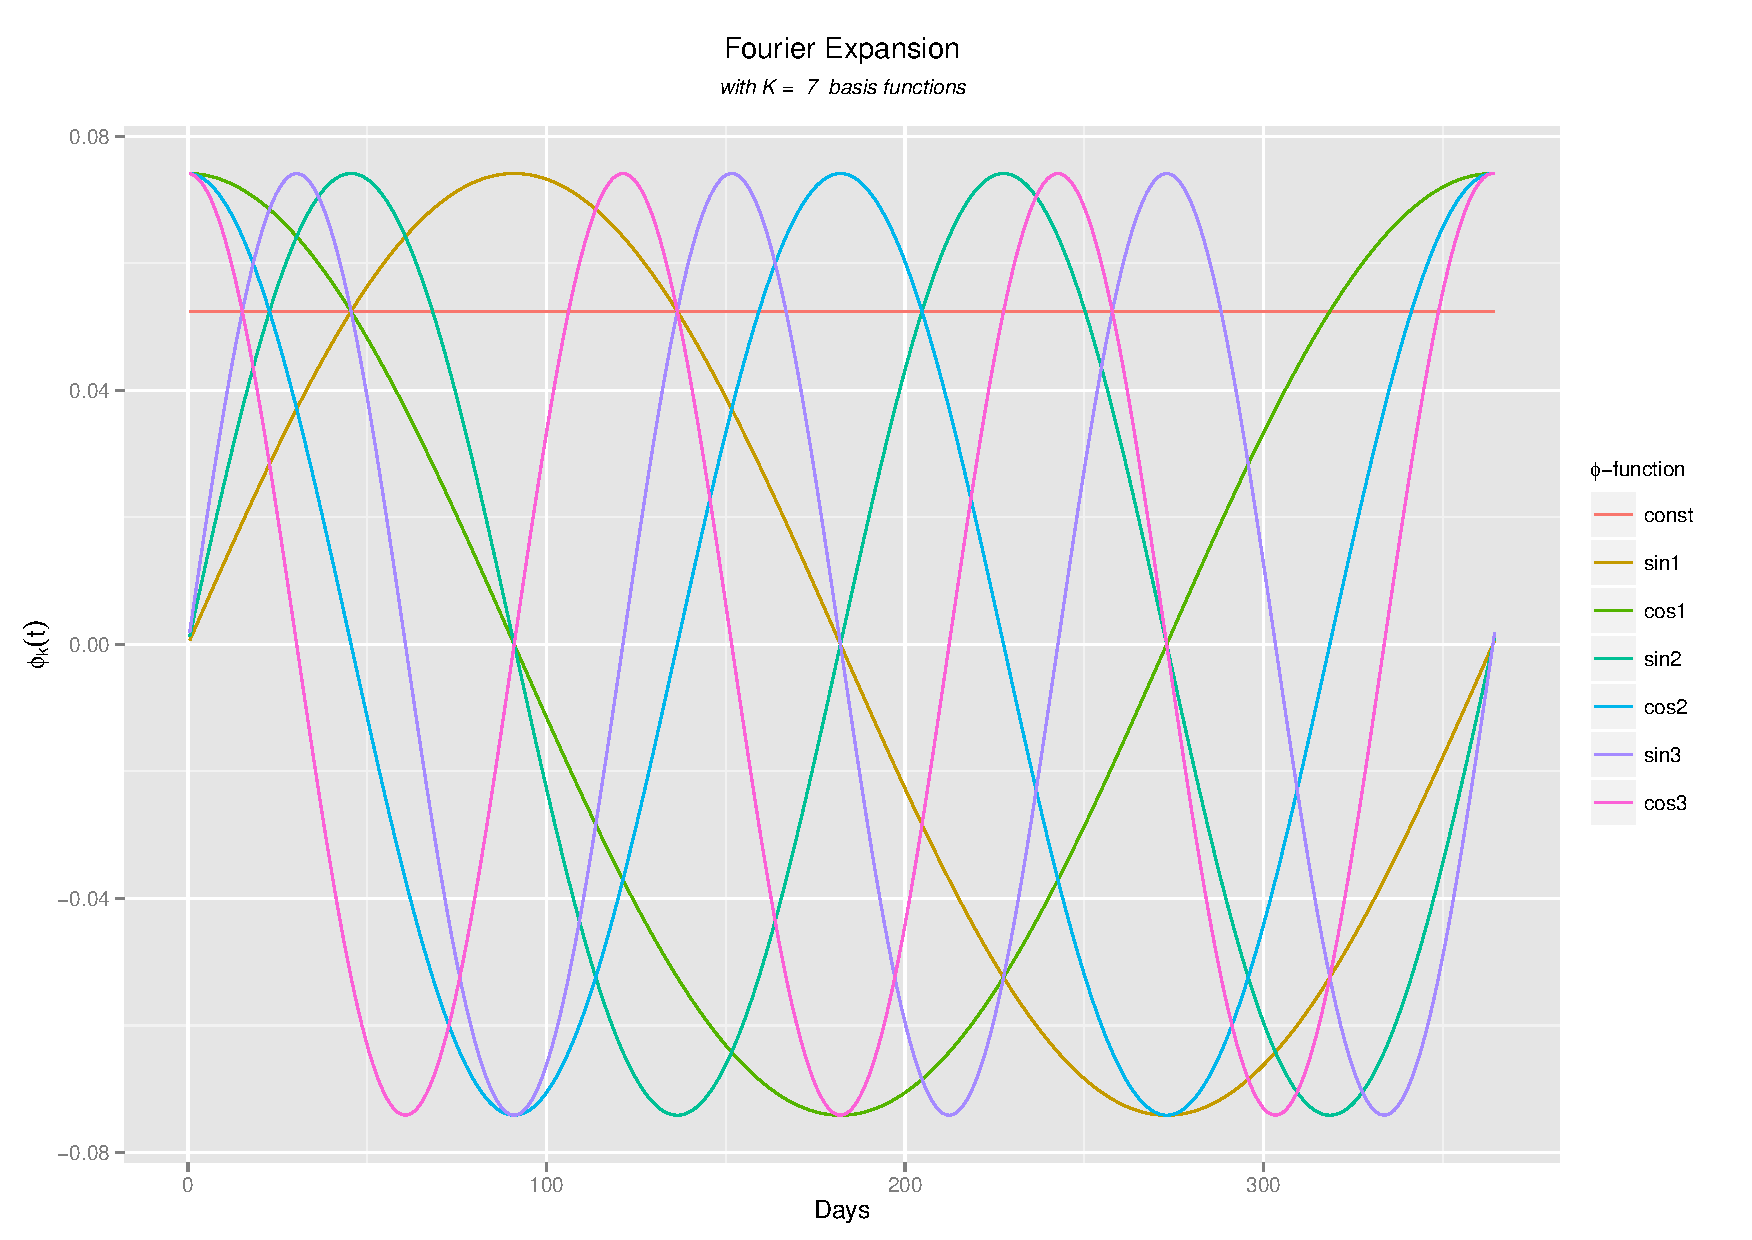
\includegraphics[height=9cm, width=1\textwidth]{Figures/FourierK7.pdf}
%    \rule{35em}{0.5pt}
  \caption[\textit{Fourier Basis} with \textit{K}=7.]{\textit{Fourier Basis} defined over the interval $\left[0,365\right]$.}
  \label{fig:FDA2}
\end{figure}

\begin{figure}[h]
  \centering
    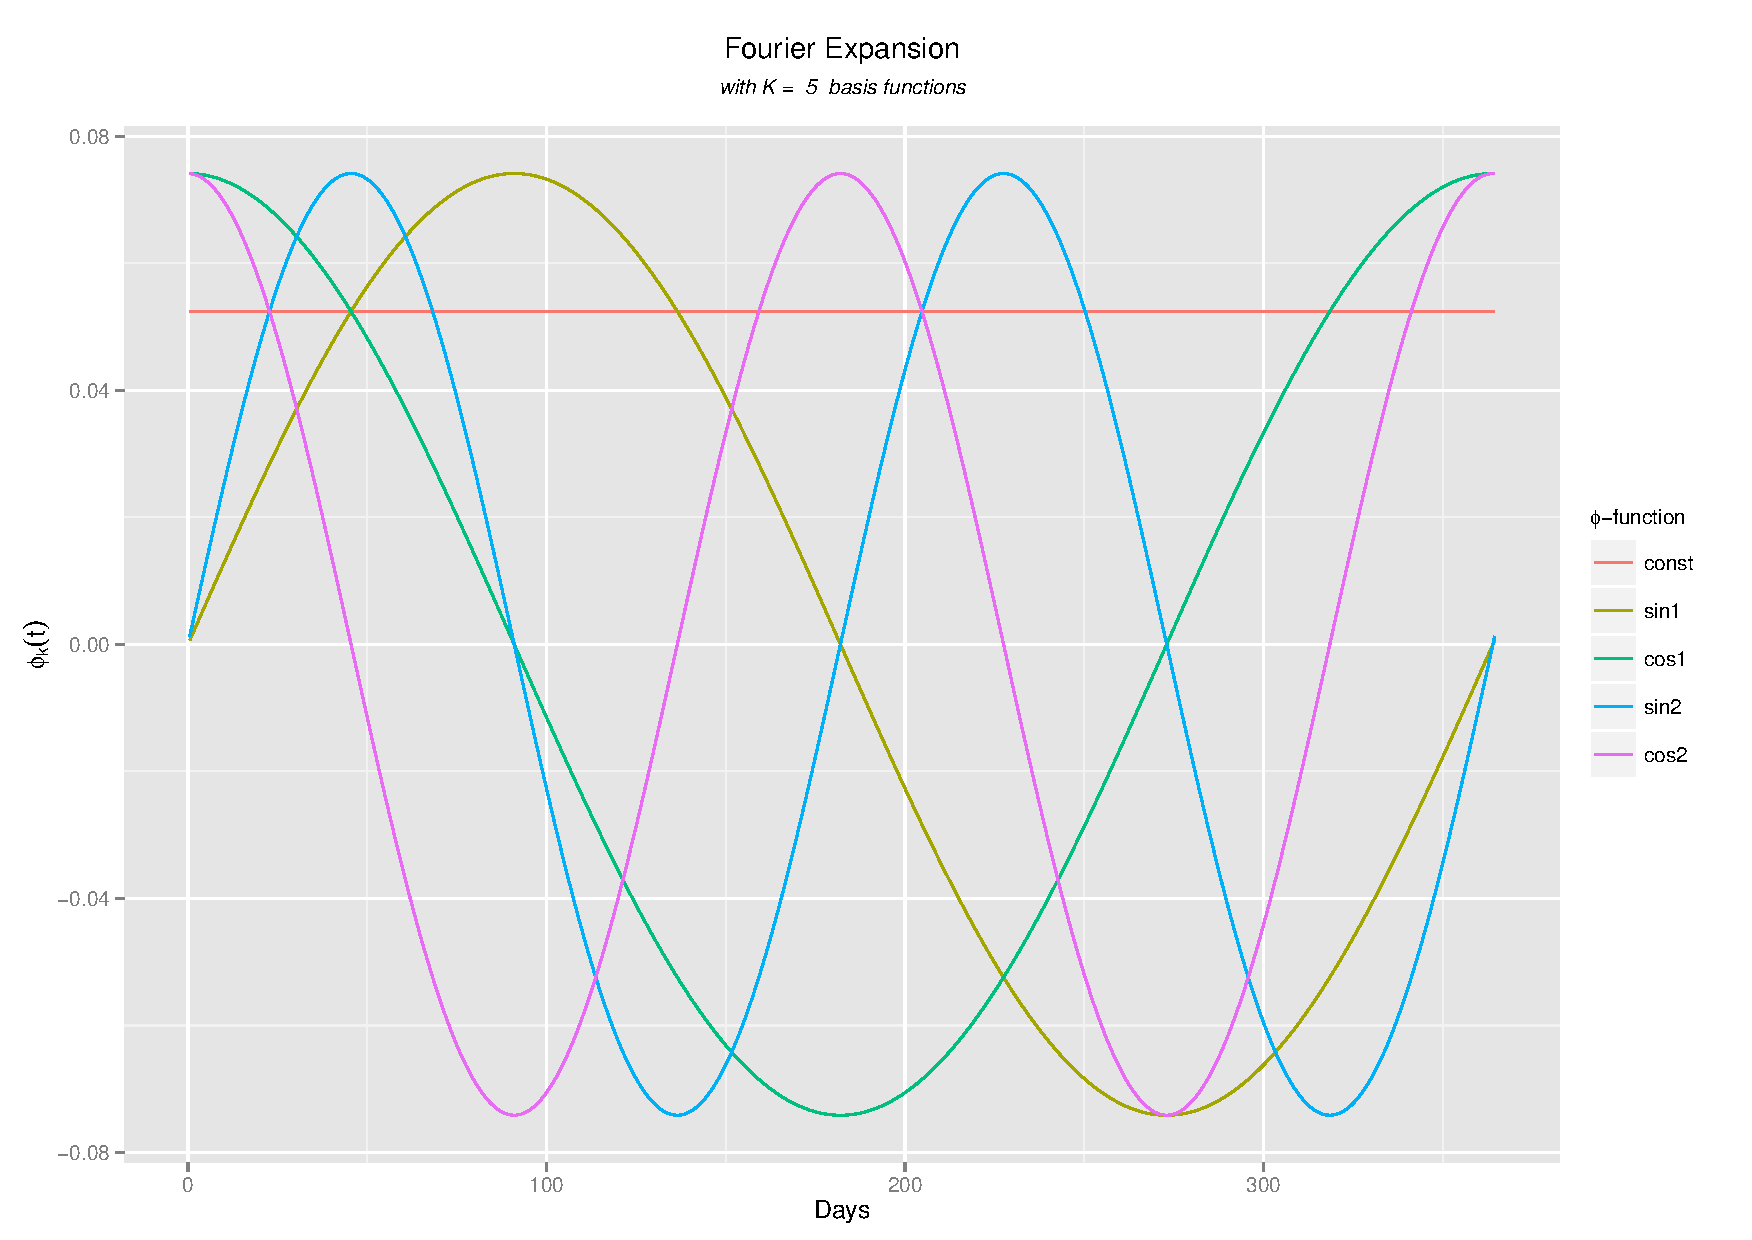
\includegraphics[height=9cm, width=1\textwidth]{Figures/FourierK5.pdf}
%    \rule{35em}{0.5pt}
  \caption[\textit{Fourier Basis} with \textit{K}=5.]{\textit{Fourier Basis} defined over the interval $\left[0,365\right]$.}
  \label{fig:FDA11}
\end{figure}

Figure~\ref{fig:FDA112} illustrates the smoothing of the \textit{Temperature} data in the \texttt{Oviedo} using a \textit{Fourier Basis} with $K = 121$, $K = 51$ and $K = 5$.

\begin{figure}[h]
  \centering
    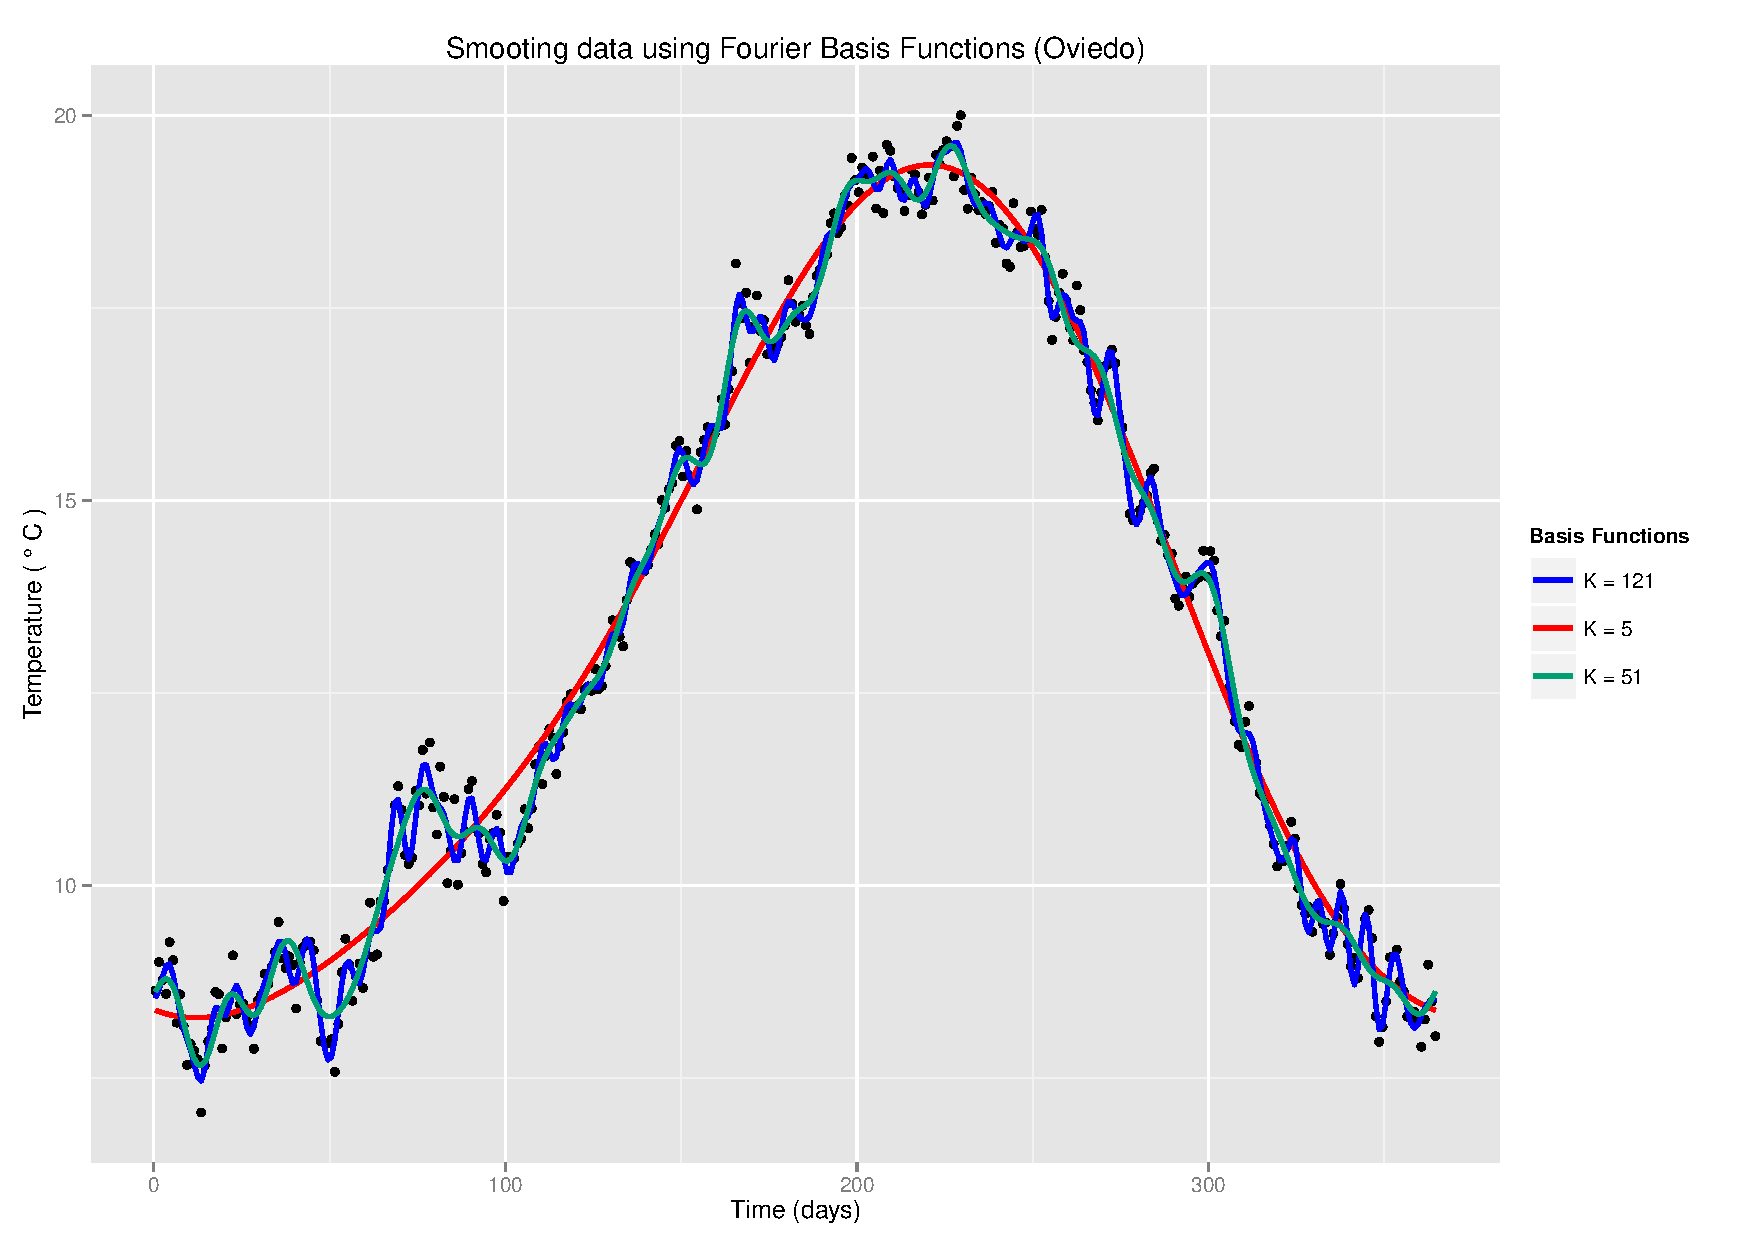
\includegraphics[height=9cm, width=1\textwidth]{Figures/Fourier_Oviedo.pdf}
%    \rule{35em}{0.5pt}
  \caption[\textit{Fourier Basis} applied on Oviedo Temperature data]{\textit{Fourier Basis} applied on Oviedo Temperature data $\left[0,365\right]$.}
  \label{fig:FDA112}
\end{figure}  
\\
\subsection{B-Splines Basis}
Originally derived by \cite{DeBoor2001}, the set of basis splines is a well-known \textit{Functional Basis} for non-periodic data. They are linear combinations of spline functions of specified order over a specified number of breakpoints. A spline is a piecewise polynomial function of order \textit{m} over each interval, which is smoothly connected at breakpoints. More precisely, the interval $\mathcal{T}$ on which the basis is defined is divided into $L$ subintervals separated by values $\tau_{l}, l=0,\dots,L$ called breakpoints or knots. Let $B_{k,m}(t)$ denote the $k$-th \textit{B-Splines Basis} function of order $m$ defined for any value of $t$, for the non-decreasing sequence of knots $\{ \tau_{l} \}_{l=0}^{L}$.
\vskip
\setlength{\parindent} In this case, $\phi_{k}(t)$ is defined as follows:
\begin{equation}
\phi_{k}(t)= B_{k,m}(t),\text{ }\forall t \in \mathcal{T},\text{ } k=1,\dots,m+L-2
\end{equation}

Let $\xi_0 < \xi_1$ and $\xi_K < \xi_{K+1}$ be two boundary knots defining the domain over which the spline is evaluated. The augmented knot sequence $\tau$ is defined as:

\begin{itemize}
\item $\tau_1 \leq \tau_2 \leq \dots \leq \tau_M \leq \xi_0$;
\item $\tau_{j+M} = \xi_j, \text{ }j = 1,\dots,K$;
\item $\xi_{K+1} \leq \tau_{K+M+1} \leq \tau_{K+M+2} \leq \dots \leq \tau_{K+2M}$.
\end{itemize}
Any additional knots beyond the boundary are abitrary, and the usual scenario is to make them all the same an equal to $\xi_0$ and $\xi_{K+1}$.
The set of basis functions $B_{k,m}(t)$ of order $m$ for the knot-sequence $\tau$ (where $m < M$) is derived using a recursion formula as follows:

\begin{eqnarray}
B_{k,1}(t) = \left\{ 
\begin{array}{cc}
1, & \quad \textrm{ } t\in [\tau_{l},\tau_{l+1}]\\
0, & \quad \textrm{otherwise}
\end{array}\right.
\end{eqnarray}
for $k = 1,\dots,K+2M-1$. These functions are called Haar basis functions. 
\begin{equation}
B_{k,m}(t)=\frac{t-\tau_{l}}{\tau_{k+m-1}-\tau_{k}}B_{k,m-1}(t)+\frac{\tau_{k+m}-t}{\tau_{k+m}-\tau_{k+1}}B_{k+1,m-1}(t),\text{ }\forall t \in \mathcal{T},\text{ } m \geq 2 .
\end{equation} for $k = 1,\dots,K+2M-m$.
In this case, the function vector $\bm{\phi}(t)$ defined in equation~\eqref{fda_23} has $K+2M-m$ basis functions evaluated at discrete time points $t_{j}, \text{ where }j=1,\dots,J$. \\In other words, the number of basis functions is defined by its order and its number of knots. The main advantages of the \textit{B-Splines Basis} are its flexibility as well as its fast computation.

\begin{figure}[h]
  \centering
    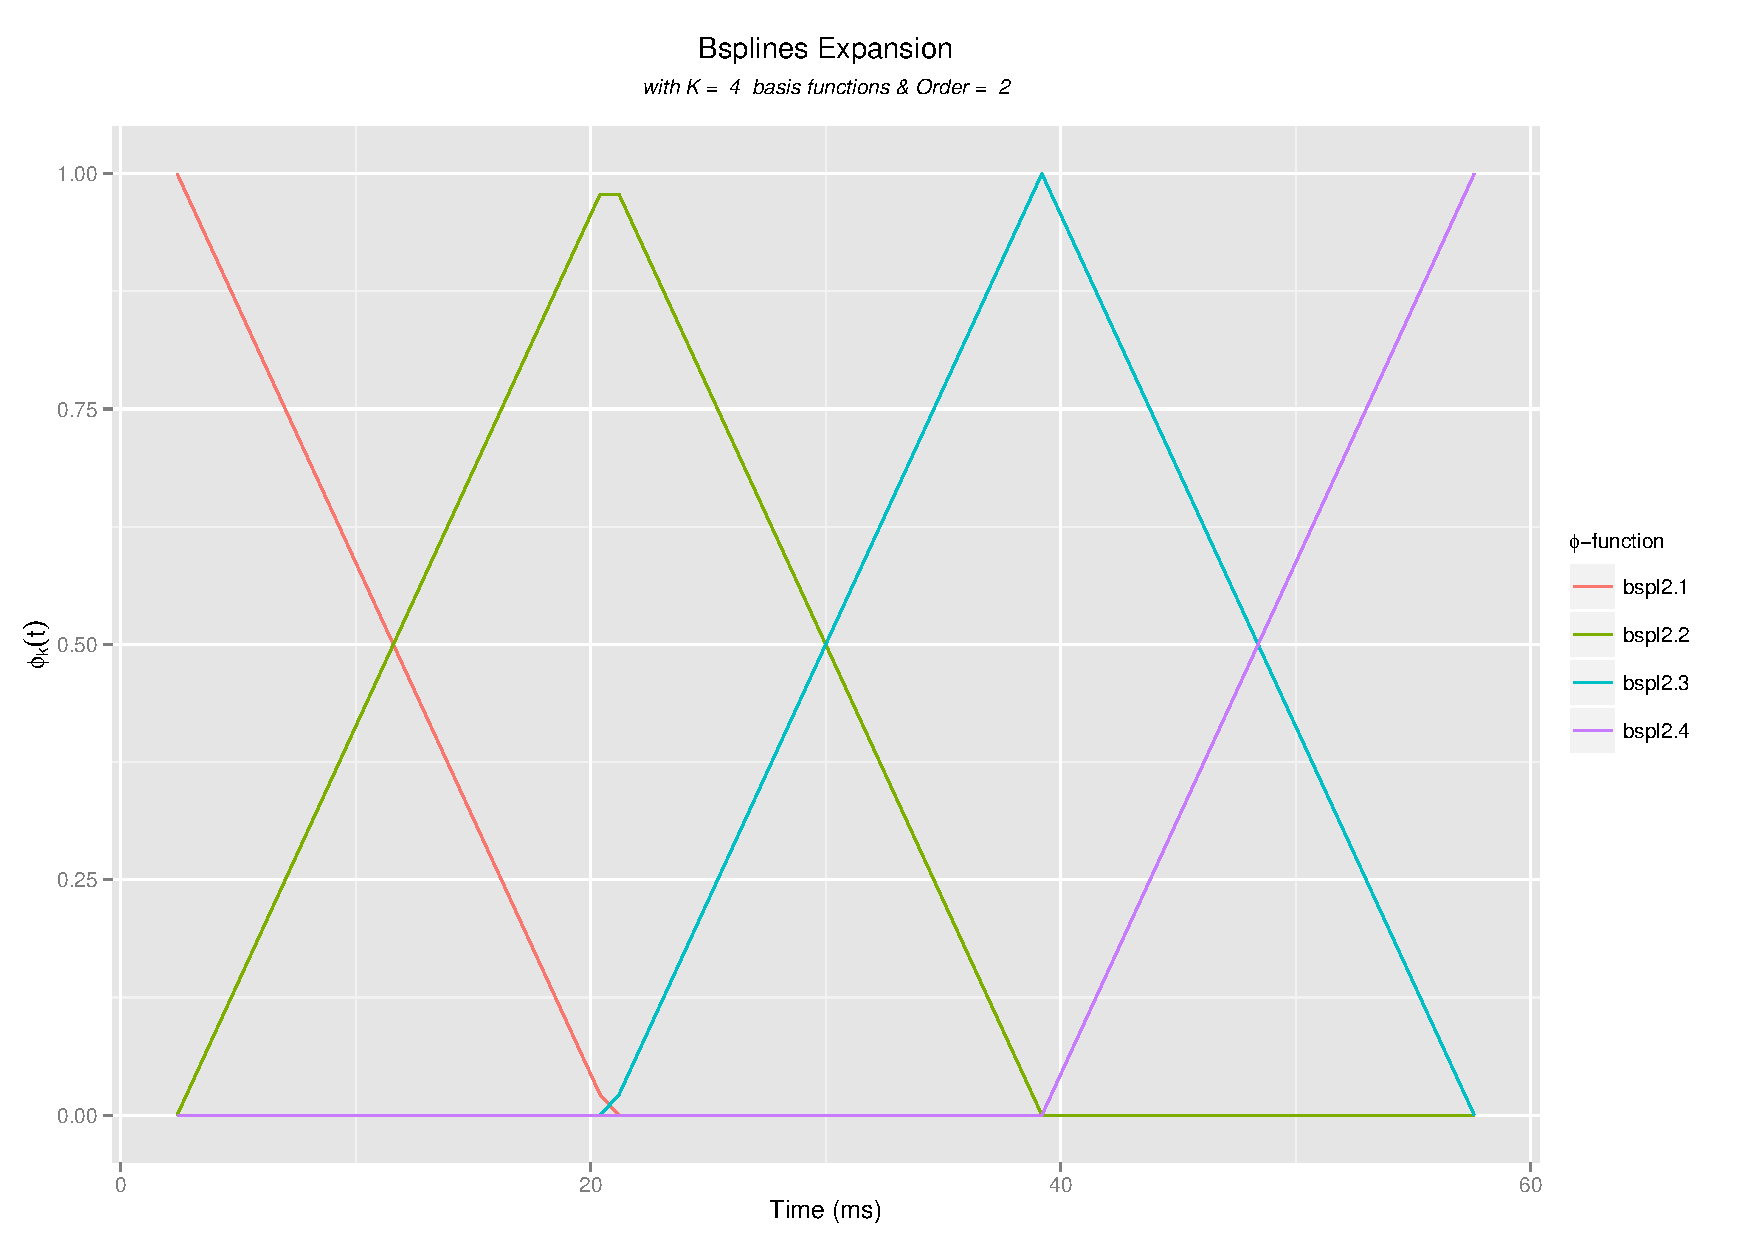
\includegraphics[height=9cm, width=1\textwidth]{Figures/BsplineK4o2.pdf}
%    \rule{35em}{0.5pt}
  \caption[\textit{B-Splines Basis} of order 2 with 4 basis functions]{\textit{B-Splines Basis} of order 2 with 4 basis functions}
  \label{fig:FDA3}
\end{figure}
%\clearpage

\begin{figure}[h]
  \centering
    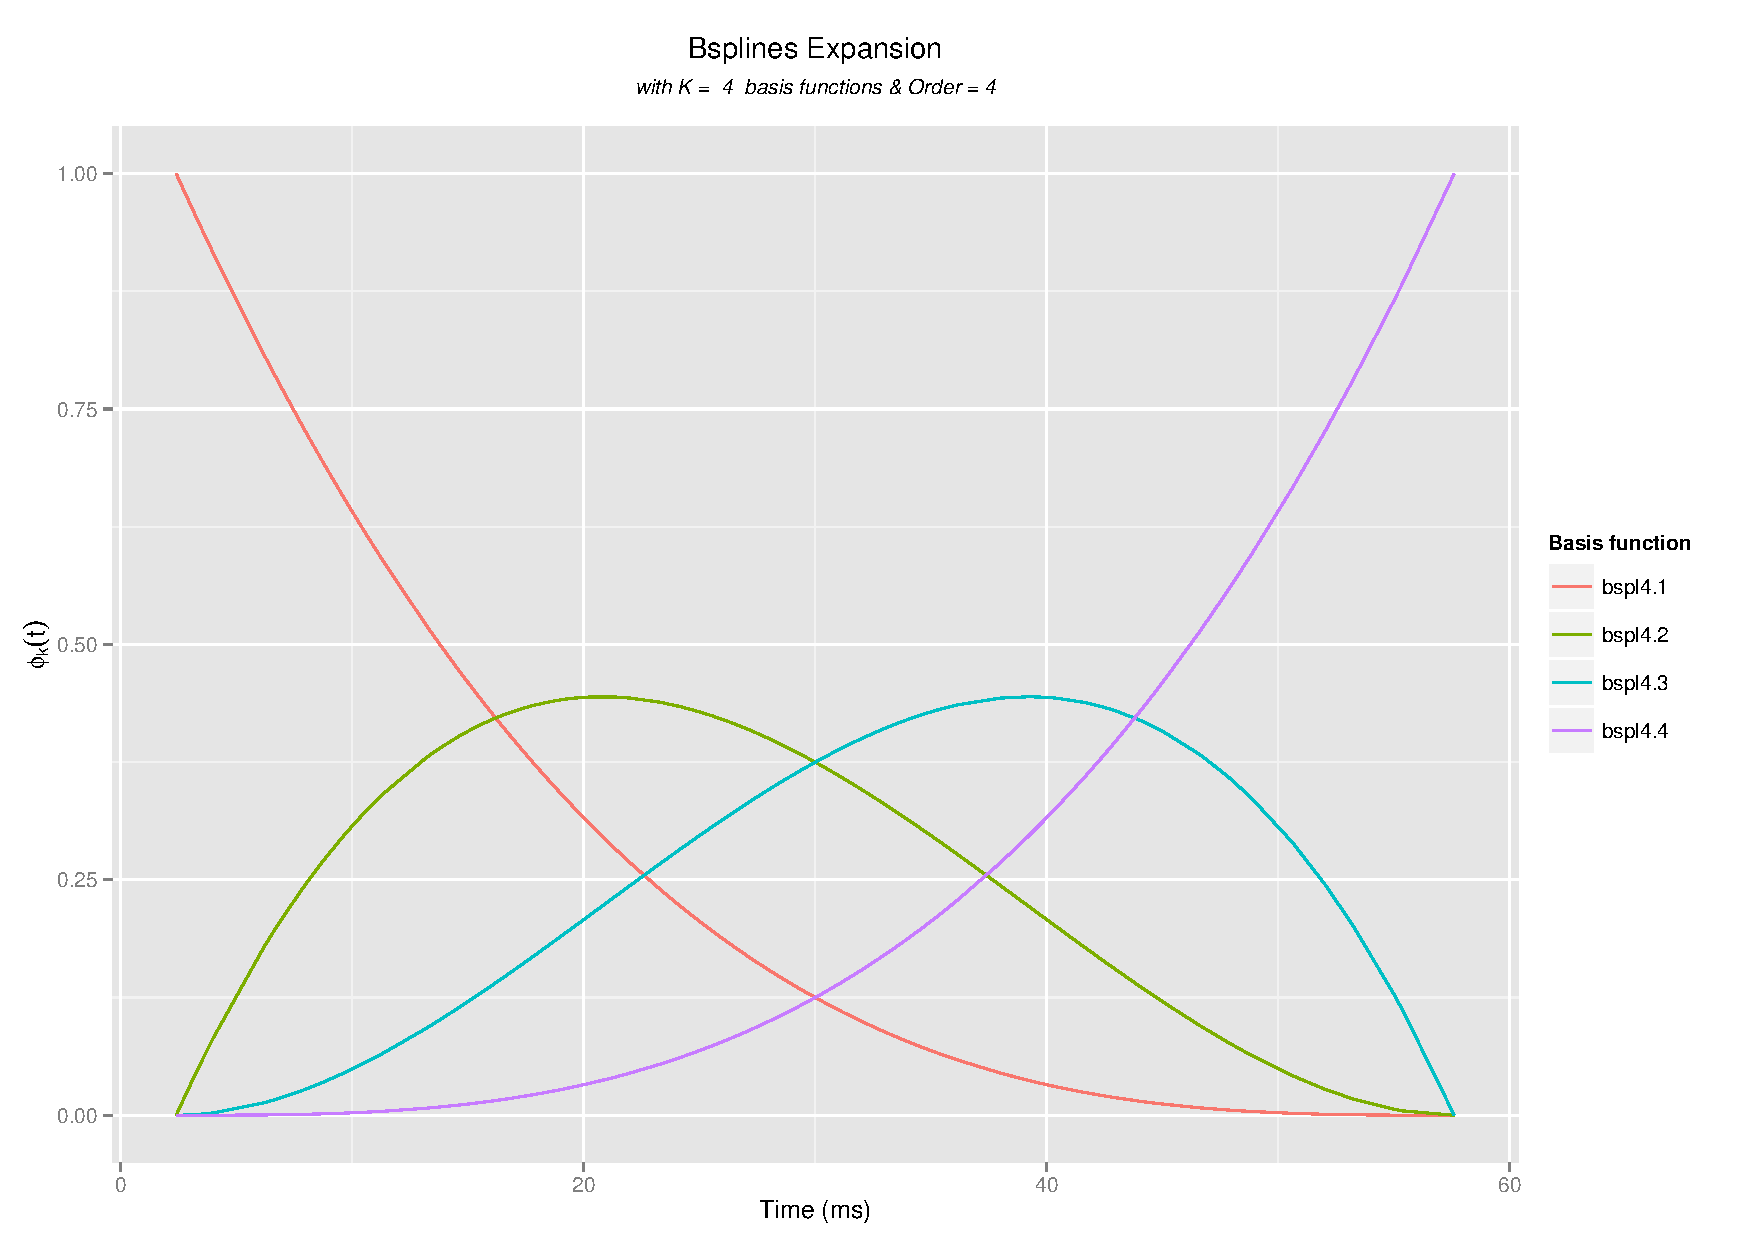
\includegraphics[height=9cm, width=1\textwidth]{Figures/BsplineK4o4.pdf}
%    \rule{35em}{0.5pt}
  \caption[\textit{B-Splines Basis} of order 4 with 4 basis functions]{\textit{B-Splines Basis} of order 4 with 4 basis functions}
  \label{fig:FDA41}
\end{figure}
\clearpage

Smoothed estimates of the observed data are derived when applying this smoothing technique onto a non-periodic dataset, but it depends on the parameter $K$. For illustration, consider the \texttt{Motorcycle Data} which has been widely used by \citet{Silverman1985} and \citet{Hardle94}. For more information on the dataset, refers to the \texttt{R}-package \texttt{adlift} created by \cite{Motordata}. Figure~\ref{fig:FDA42} depicts the \texttt{Motorcycle Data} smoothed with the \textit{B-Splines} function for $K = 20$ and $K = 40$. 

\begin{figure}[h]
  \centering
    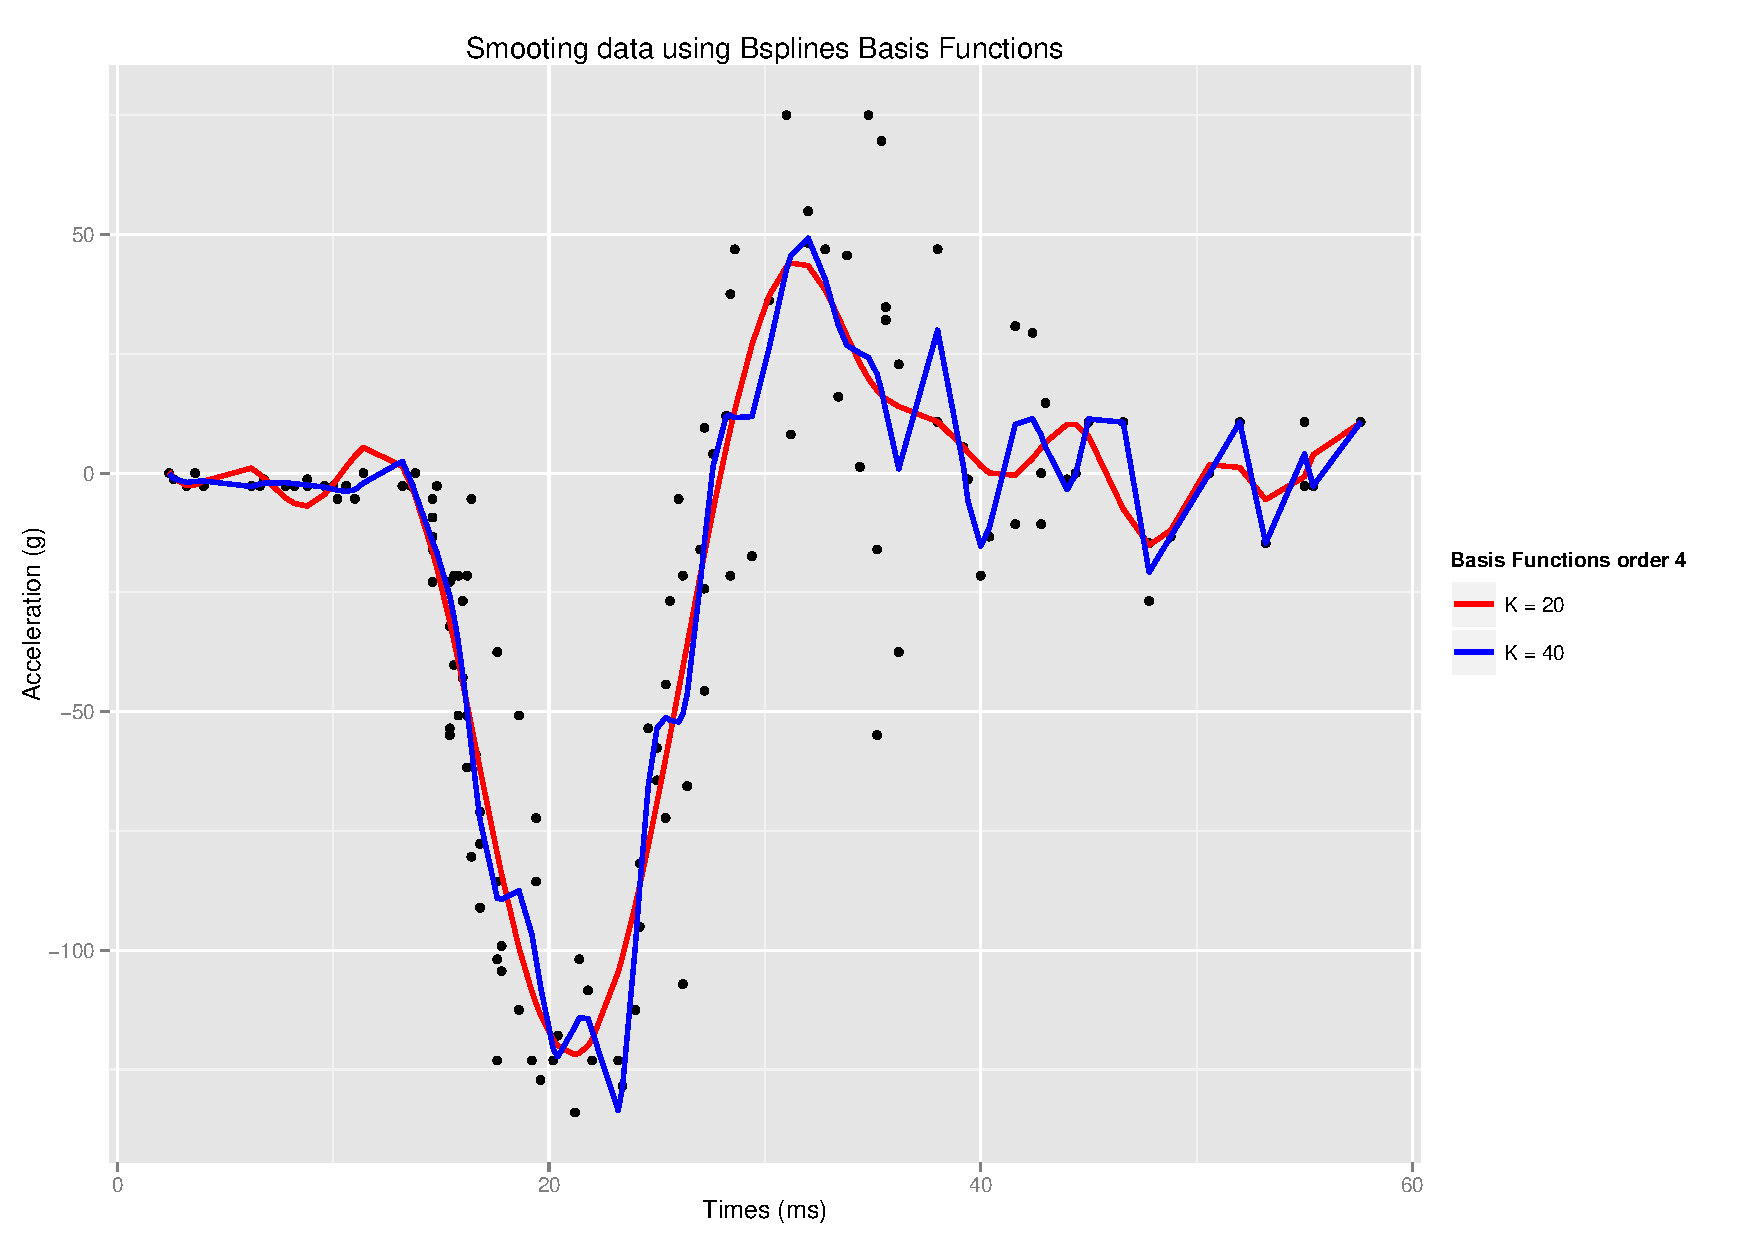
\includegraphics[height=9cm, width=1\textwidth]{Figures/Bsplines_Motorcycle1.pdf}
%    \rule{35em}{0.5pt}
  \caption[\textit{B-Splines Basis} Basis applied on the \texttt{Motorcycle Data}]{\textit{B-Splines Basis} Basis applied on the \texttt{Motorcycle Data}}
  \label{fig:FDA42}
\end{figure}

\subsection{Gaussian Radial Basis Functions}

Radial basis functions is a class of single hidden layer feedforward networks which can be expressed as a linear combination of radially symmetric nonlinear basis functions \citep{Ando2008}. Each basis function forms a localized receptive field in the input space. The most commonly used function is the \textit{Gaussian Basis} functions which is given by:

\begin{equation}
\phi_k(t;\mu_k ,\sigma^2_k) = \exp \left(-\dfrac{||t-\mu_k||^2}{2\sigma^2_k}\right),\textbf{ } k=1,\dots,K
\end{equation}
where $\mu_k $ is a parameter determining the center of the basis function, $\sigma^2_k $ is a parameter that determines the width and $||.||$ is the Euclidian norm. \textit{Gaussian Basis} functions have a number of useful analytical and practical properties (see \cite{Bishop1995}). The basis functions overlap with each other to capture the information about \textbf{t}. More importantly, the width parameter play an essential role to capture the structure in the data over the region of input data. The parameters featuring in each basis function are often determined heuristically based on the structure of the observed data.\\
\cite{Moody1989} used the \texttt{K-means} clustering algorithm to determine both the center and the width parameter of the basis function. This algorithm splits the observational space $\mathcal{T}$ into $K$ clusters $\{C_1,C_2,\dots,C_K\}$ that correspond to the number of basis functions. They are determined by:
\begin{equation}
\hat{\mu}_k = \frac{1}{N_k}\sum_{t_j \in C_k} t_j, \text{  } \hat{\sigma}^2_k = \dfrac{1}{N_k}\sum_{t_j \in C_k} ||t_j - \hat{\mu}_k||^2,
\end{equation}

where $N_i $ is the number of observations which belongs to the $k^{th}$ cluster. However, this method does not produce unique parameters for a unique set of observations, due to the stochastic nature of the starting value in the clustering algorithm. Because of that feature, the \textit{K-means} clustering underperforms when capturing all the information from the data. This is noticeable when the set of Functional Data are observed at equidistant points.\\ \cite{Ando2008} proposed to include the hyper-parameter $\nu$ ($> 0$) to control the amount of overlapping as a mean to overcome the lack of overlapping among basis functions. The transformed \textit{Gaussian Basis} are now given by:

\begin{equation}
\phi_k(t;\mu_k ,\sigma^2_k) = \exp \left(-\dfrac{||t-\mu_k||^2}{2\nu \sigma^2_k}\right),\textbf{ } k=1,\dots,K
\end{equation}

In order to stabilize the estimation of the Gaussian basis functions parameters, \cite{kawano2007} proposed basis functions where the centers and the width parameters are determined by preassigned knots similar to \textit{B-Splines} basis functions. Consider the observations $\{x_j;\text{ } j=1,\dots,n\}$ arranged by magnitude, the knots $t_k\text{ }(k = 1,\dots,K+4)$ are set up as follows:
\begin{equation}
t_1 < t_2 < t_3 < t_4 = x_1 < t_5 < \dots < t_K < t_{K+1} = x_K < t_{K+2} < t_{K+3} < t_{K+4}
\end{equation}
where the knots are equally spaced. By setting the knots in this way the \textit{n} observations are divided into $(K-3)$ intervals:

\begin{equation}
[t_4,t_5],[t_5,t_6],\dots,[t_K,t_{K+1}].
\end{equation}
The \textit{Gaussian Basis} functions are now defined with a center $t_k$ and a width $h = (t_k - t_{k-2})/3$ for $k = 3,\dots,K+2$ as follows:
\begin{align} 
\begin{split}
\phi_k(x;t_k ,h^2) &= \exp \left(-\dfrac{||x-t_k||^2}{2 h^2}\right)\\
h 	&= \dfrac{t_k - t_{k-2}}{3}, \text{  } k = 3,\dots,K+2\\
\end{split}					
\end{align}

Figure~\ref{fig:FDA45} shows two different \textit{Gaussian Basis} functions (with 8 functions) plotted on the same set of observations. Note that the areas under the curves for \textit{K-means} clustering are different, whereas the areas for \textit{Gaussian Basis} using \textit{B-Splines} approach are consistent.

\begin{figure}[h]
  \centering
    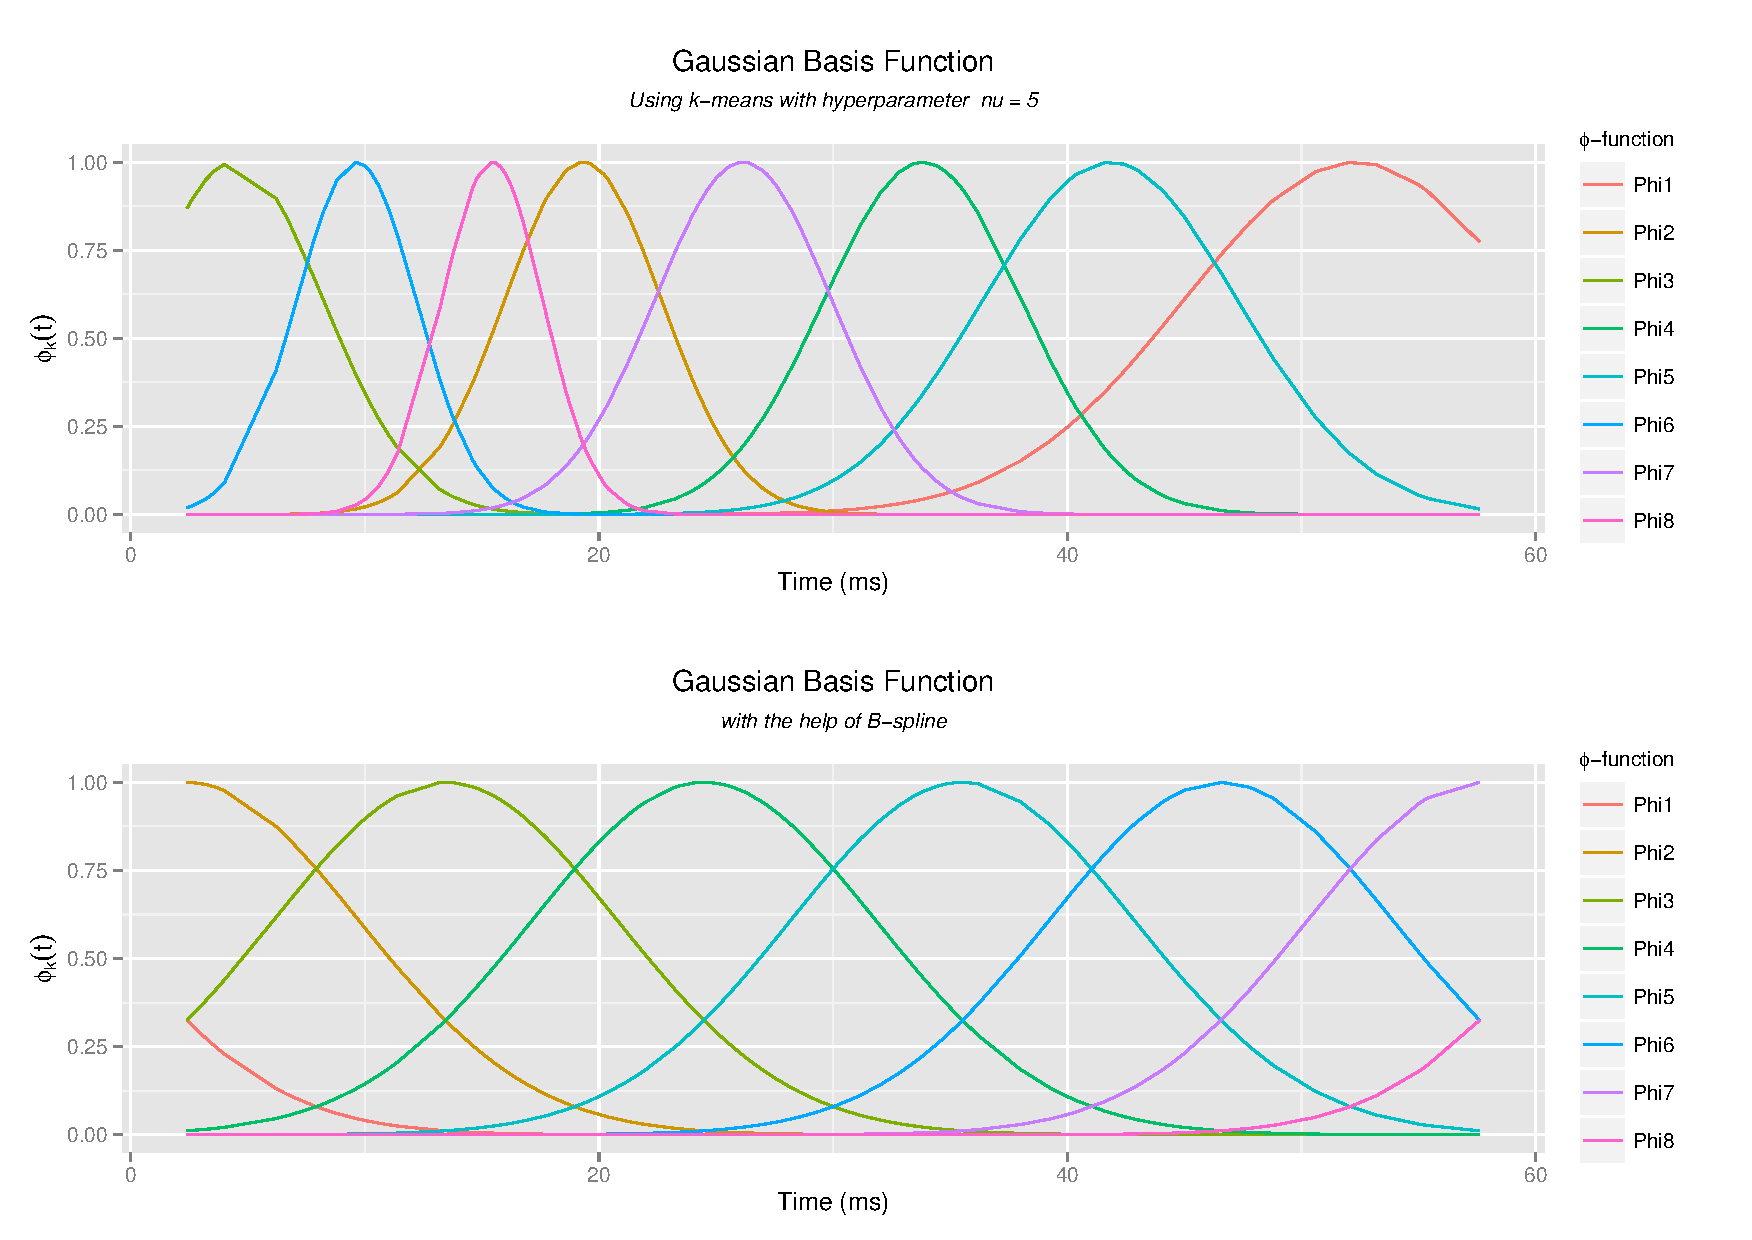
\includegraphics[height=14cm, width=1\textwidth]{Figures/gaussian_motor1.pdf}
%    \rule{35em}{0.5pt}
  \caption[Contrast between \textit{K-means} clustering method and \textit{B-Splines} method]{Contrast between \textit{K-means} clustering method and \textit{B-Splines} method}
  \label{fig:FDA45}
\end{figure}
\clearpage
Figure~\ref{fig:FDA4} shows smooth curves obtained when applying the abovementioned methods on the motorcycle impact data using the following basis functions: (1)\textit{Gaussian Basis} using \textit{B-Splines} (K = 20);  (2) \textit{Gaussian Basis} using \textit{K-means} (K = 20, $\nu = 2$).

\begin{figure}[h]
  \centering
    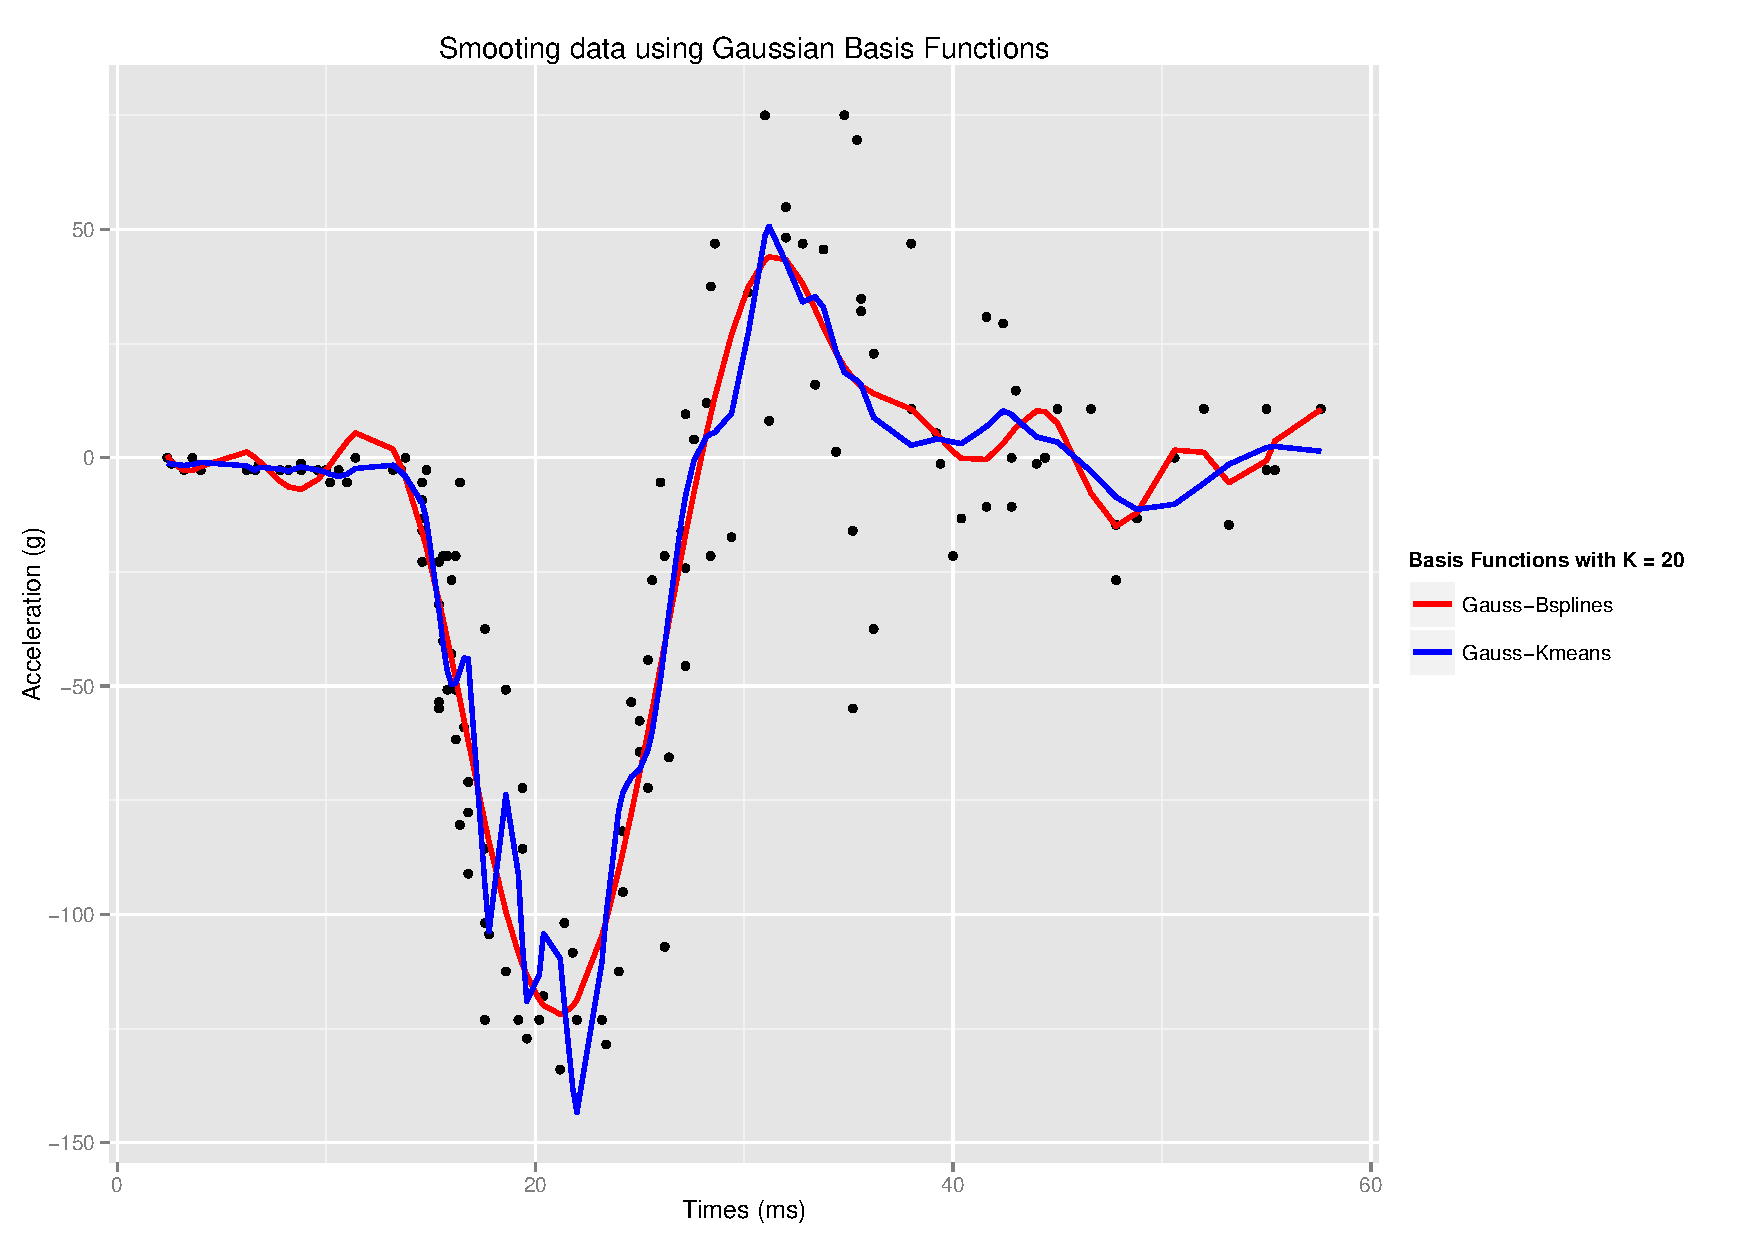
\includegraphics[height=9cm, width=1\textwidth]{Figures/gauss_motorcycle2.pdf}
%    \rule{35em}{0.5pt}
  \caption[Motorcyle impact data fitted with  \textit{Gaussian Basis} functions]{Motorcyle impact data fitted with \textit{Gaussian Basis} functions}
  \label{fig:FDA4}
\end{figure}


\subsection{Other Basis Functions}

Recent developments in the study of Functional Data have led to a number of other potentially important basis systems. For instance, the \textit{Haar Wavelets} which combine the frequency-specific approximating power of the \textit{Fourier Basis} with the time- or spatially-localized features of \textit{Splines}. Another example, \textit{Simple Bases} such as step functions and polynomial bases:
\subsubsection*{Haar Wavelets}
The \textit{Haar Wavelets} transform is useful to model a multiresolution stochastic process. It exploits the idea that a basis is constructed by choosing a suitable scaling function $\phi$ (the \textit{Father Wavelet}) and the function $\psi$ (the \textit{Mother Wavelet}) of the \textit{Haar Wavelets} defined on $[0,1)$. The functions $\phi(t)$ and $\psi(t)$ are given by:
\begin{center}
$\phi(t) =
    \begin{cases}
            1, &         \text{if } 0 \leq t < 1;\\
            0, &         \text{if otherwise};
    \end{cases}$
\end{center}

\begin{center}
$\psi(t) =
    \begin{cases}
            1, &         \text{if } 0 \leq t < 1/2;\\
            -1, &         \text{if } 1/2 \leq t < 1;\\
            0, &         \text{if otherwise}.
    \end{cases}$
\end{center}
The Haar wavelets are then generated in the form of translations and dilations of the above father and mother wavelet functions as
\begin{align}
\phi_{j,k}(t) &= \sqrt{2^j}\phi(2^j t - k), \nonumber \\
\psi_{j,k}(t) &= \sqrt{2^j}\psi(2^j t - k), \nonumber
\end{align}

where $j = 0,1,\dots$ and $k = 0,1,\dots,2^j -1$. The index $j$ refers to dilations and $k$ refers to translations and $\sqrt{2}$ is the normalizing factor. The mother wavelet is constructed to ensure that the basis is orthogonal. The \textit{Wavelet Basis} idea is easily adapted to deal with functions defined on a bounded interval, most simply if periodic boundary conditions are imposed \citep{olberd:ramsay}. The coefficients of $\psi_{jk}$ yield information about $f$ near position $2^{-j}k$ on scale $2^{-j}$. In contrast to \textit{Fourier Basis}, \textit{Wavelet Basis} expansions cope well with discontinuities and rapid changes in behavior, that allows them to accomodate a wide variety of functional forms. See \cite{walker2008} for more details on \textit{Wavelet Basis}.
\subsubsection*{Polynomial bases}
The basis functions could be expressed as $\phi_{k}(t)=\left(t-\omega\right)^{k},\text{ }\forall t \in \mathcal{T}, \text{ }k=0,\dots,n$, where $\omega$ is a shift parameter that is usually chosen to be in the center of the interval of approximation. Like the \textit{Fourier Basis} expansion, \textit{Polynomials Basis} cannot exhibit local features without using a large number of basis functions. They tend to fit well in the center of the data but exhibit rather unattractive behavior around the tails. Although derivatives of \textit{Polynomials Basis} expansion are simple to compute, they are usually a poor basis for extrapolation or forecasting.

\subsubsection*{Kernel Smoothing}
Smoothing problems, in a statistical framework, are appropriate under the consideration that the data set is merely a realization of a random sample from a certain population. For a smoothing method to make sense, the value of the function estimated at a point $\phi(t_{j})$ must be influenced mostly by the observations near that point. An intuitive estimator $\hat{\phi}_{i}(t)$ is the locally weighted average. Generally speaking a kernel smoother defines a set of weights $\{W_{i}^{h}(t)\}^{n}_{i=1}$ for each $t$.
Let $\mathcal{K}$ be a real-valued function assigning weights. The function $\mathcal{K}$, also called the \textit{Kernel} function, is usually a symmetric probability density. Let $h$ be a bandwidth which is a nonnegative number controlling the size of the local neighborhood. \cite{olberd:ramsay} described the \textit{Kernel Basis} as a function that has most of its mass concentrated close to 0, and either decay rapidly or disappear entirely for $|u| \geq 1$. The most popular \textit{kernel} functions are:
\begin{itemize}
\item \textbf{Gaussian:} $\mathcal{K}(u)=\dfrac{1}{\sqrt{2\pi}}\text{exp}\left[-u^{2}/2\right]$
\item \textbf{Epanechnikov:} $\mathcal{K}(u)= \dfrac{3}{4} \mathbbm{1}_{\left[-1,1\right]}(1-u^{2})$
\item \textbf{Triweigth:} $\mathcal{K}(u)= \dfrac{35}{32} \mathbbm{1}_{\left[-1,1\right]}(1-u^{2})^{3}$
\item \textbf{Uniform:} $\mathcal{K}(u)= \dfrac{1}{2} \mathbbm{1}_{\left[-1,1\right]}(u)$
\item \textbf{Cosine:} $\mathcal{K}(u)= \dfrac{\pi}{4} \mathbbm{1}_{\left[-1,1\right]}\cos(\pi \times u/2)$
\item \textbf{Quartic:} $\mathcal{K}(u)=\dfrac{15}{16} \mathbbm{1}_{\left[-1,1\right]}(1-u^{2})^{2}$ 
\end{itemize}
The estimate at a given point is a linear combination of local observations,
\begin{equation*}
\hat{\phi}_{i}(t) = \sum\limits_{j=1}^{p}\hat{W}_{i}^{h}(t_{j})Y_{j}
\end{equation*}
for some suitably defined weight functions $W^{h}(t_{j})$. \citet{Nada1964} and \citet{Wats1964} developed one of the most popular kernel estimator the \textit{Nadaraya-Watson} estimator given by:
\begin{equation}
\hat{W}^{h}(t_{j})=\frac{\sum\limits_{j=1}^{p}\mathcal{K}^{h}(t_{j}-t)Y_{j}}{\sum\limits_{j=1}^{p}\mathcal{K}^{h}(t_{j}-t)}
\end{equation}
where $\mathcal{K}^{h}(.)=\mathcal{K}(./h)/h$. \cite{Gasser1979,GassMull1984} constructed the weights as follows:
\begin{equation}
\hat{W}^{h}(t_{j})=\sum\limits_{j=1}^{p}\int\limits_{\bar{t}_{j}}^{\bar{t}_{j-1}}\mathcal{K}^{h}(u-x)du \times Y_{j}
\end{equation}
with $\bar{t}_{j}=(t_{j+1}+t_{j})/2$, $1 \leq j \leq n$, $\bar{t}_{0} = t_{1}$ and $\bar{t}_{p} = t_{p}$. This estimator was originally proposed for \textit{equispaced designs}, but can also be used for \textit{non-equispaced designs}. Figure~\ref{fig:FDA5} depicts a visualization of \textit{Kernel} smoothing regression.
\begin{figure}[h]
  \centering
    \includegraphics[height=8cm, width=1\textwidth]{Pictures/Untitled.png}
%    \rule{35em}{0.5pt}
  \caption[\textit{Kernel Smoothing} regression at Boundaries]{An illustration of \textit{Kernel Smoothing} regression technique (Image taken from \citealp{hastie_09_elements-of.statistical-learning})}
  \label{fig:FDA5}
\end{figure}

\subsubsection*{Local Polynomials Fitting}
Local polynomials fitting was originally proposed by \cite{Clev:1979} and further developed by \cite{Fan:Gijb:1995}. Consider the bivariate data $(t_{1},Y_{1}),\dots,(t_{p},Y_{p})$, an i.i.d. sample from a population. The interest is in estimating the regression function $\hat{\phi}(t_{0})$ and its derivatives $\hat{\phi}'(t_{0}),\hat{\phi}''(t_{0}),\dots,\hat{\phi}^{(m)}(t_{0})$. 
The unknown regression funtion $X(t)$ is approximated locally by a polynomial of order \textit{p} at the point $t_{0}$. A Taylor expansion in a neighborhood of $t_{0}$, gives:
\begin{equation}\label{eq:taylorex}
\phi(t) \approx \phi(t_{0}) + \phi'(t_{0})(t-t_{0}) + \frac{\phi''(t_{0})}{2!}(t-t_{0})^{2}+\dots+\frac{\phi^{(m)}(t_{0})}{m!}(t-t_{0})^{m}.
\end{equation}
This polynomial is fitted locally by a weighted least squares regression problem: minimize
\begin{equation}\label{eq:leastsq}
\text{min}\left(\sum\limits_{j=1}^{p}\{Y_{j}-\sum\limits_{k=1}^{m}\beta_{k}\left(t_{j}-t_{0}\right)^{k}\}^{2}\mathcal{K}^{h}(t_{j}-t_{0})\right)
\end{equation}
where \textit{h} is a bandwidth controlling the size of the local neighborhood and $\mathcal{K}^{h}(.) = \mathcal{K}(./h)/h$ is the function assigning weights to each datum point. Denote by $\hat{\beta}_{k}$, $k=0,\dots,m$, the solution to the least squares problem \eqref{eq:leastsq}. \\
It is clear from the Taylor expansion in \eqref{eq:taylorex} that $\hat{\phi}_{k}=k!\hat{\beta}_{k}$ is an estimator for $\phi^{(k)}(t_{0})$, $k=0,1,\dots,p$. To estimate the entire function $\phi^{(k)}(.)$ we solve the above weighted least squares equation for all points in the domain of interest. For local polynomial fitting $p-k$ should be taken to be odd as shown in \citep{Rupp:Wand:1994,Fan:Gijb:1995}. Unlike the Nadaraya-Watson and the Gasser-Muller estimators, local polynomial fitting adapts to various types of designs such as random and fixed designs, highly clustered and nearly uniform designs. With local polynomial fitting, there is an absence of boundary effects: the bias at the boundary stays automatically the same as in the interior, without specific boudary kernels.


%---------------------------------------------------------------------------------------
%	SECTION 3
%---------------------------------------------------------------------------------------

\section{Model Estimation}\label{model_est}
\cite{GreenSilverma1994} point out that a good fit to the data is not the one and only aim of curve fitting; another, often conflicting, aim is to obtain a curve estimate that does not display too much rapid fluctuation. The regularization approach assists modelling and quantifying these rapid fluctuations.\\
This section describes two different approaches for model estimation when using basis functions, namely the \textit{Least Squares} method (with and without penalty) and the \textit{Maximum Likehood} method (with and without penalty). Assessing these models consist of estimating several parameters involved in the modelling:
\begin{itemize}
\item the mulitplier of the penalty term (denoted as $\lambda$);
\item the number of basis functions (denoted as $K$);
\item some additional parameters based on the model assumptions;
\item the coefficients $c_{ik}$.
\end{itemize}
For small values of $\lambda$ the estimated curve becomes more variable since it is being penalized less for its roughness. In other words, as $\lambda \rightarrow 0$, the curve fits the discrete points exactly at almost all sampling points, leading to an interpolation problem. On the other hand, when $\lambda \rightarrow \infty$ the variability in the function $X(t)$ becomes so small that the fitted curve approaches standard linear regression.
\clearpage
\subsection{Least Squares Method}
In a Functional Data framework, the method of Least Square (LS) estimation is a standard approach that consists of minimizing the Residual Sum of Squares (RSS) with $\text{RSS}(\bm{Y}_i)=\sum_{j}^{J}\left[Y_{ij}-\sum\limits_{k}^{K}c_{ik}\phi_{k}(t_{j})\right]^{2}, \forall i \in \{1,\dots,N\}$. The $RSS$ in matrix notation is:

\begin{equation}\label{eq:leastsqpen1}
\text{RSS}(\mathbf{Y}_i)=\left(\mathbf{Y}_i-\mathbf{\Phi}\mathbf{c}_i\right)^T\left(\mathbf{Y}_i-\mathbf{\Phi}\mathbf{c}_i\right),
\end{equation}

where $\mathbf{Y}_i$ is a vector of observed functional values of length $J$ . The coefficients vector can be estimated by minimizing the $RSS$ namely $\bm{\hat{c}}_i=\left(\bm{\Phi}^T \bm{\Phi}\right)^{-1}\bm{\Phi}^T \bm{Y}_i$. Simple LS approximation is appropriate in situations where it is assumed that the residuals $\epsilon_{i}$ are independently and identically distributed with mean vector $\mu = 0$ and constant variance $\sigma_i$.\\
Unfortunately, fitting basis expansions by least squares implies clumsy discontinuous control over the degree of smoothing. The aim is to look for a model that provides a smooth approach as well as control the degree of smoothness. The basic idea of the regularization approach is similar to the \textit{Least Square} estimation except that we include a penalty term in formula~\eqref{eq:leastsqpen1}. The penalized residual sum of squares estimate is defined as:

\begin{equation}\label{eq:leastsqpen2}
\text{PRSS}_{\lambda_i}(Y_i) =\left(\mathbf{Y}_i-\mathbf{\Phi}\mathbf{c}_i\right)^T\left(\mathbf{Y}_i-\mathbf{\Phi}\mathbf{c}_i\right)+\lambda_i \times \text{PEN}_{m}(X), 
\end{equation}

where $PEN_{m}(X)$ is the integrated squared $m^{th}$ derivative of $X(t)$ namely\\
$\text{PEN}_{m}(X)=\int_{\mathcal{T}} \left[D^{m}X(s)\right]^{2}ds$ and the smoothing parameter $\lambda$ controls the roughness. \cite{Ramsay2009FDA} extended the definition of \textit{roughness} to situations where a function departs from some baseline "smooth" behavior. For periodic functions of known period that can vary in level, such as mean temperature curves, the baseline behavior can be considered to be shifted sinusoidal variation. The \textit{harmonic acceleration operator} also called \textit{differential operator} is the function defined by $L=\omega^2 D + D^3$. For more details on \textit{harmonic acceleration operator}, interested readers should refer to \cite{olberd:ramsay}.\\
The roughness penalty $PEN_{m}(X)$ is re-expressed in matrix terms as:
\begin{align}
    \text{PEN}_{m}(X)&=\int_{\mathcal{T}} \left[D^{m}X(s)\right]^{2} ds \nonumber \\
                    &=\int_{\mathcal{T}} \left[\mathbf{c}'D^{m}\bm{\phi}(s)D^{m}\bm{\phi}^T(s)\mathbf{c}\right]ds \nonumber \\
                    &=\mathbf{c}'\int_{\mathcal{T}} \left[D^{m}\bm{\phi}(s)D^{m}\bm{\phi}^T(s)ds\right]\mathbf{c} \nonumber\\
                    &=\mathbf{c}^T \mathbf{R}\mathbf{c}\label{Rmat1}
    \end{align}

where  
\begin{equation}\label{Rmat2}
\mathbf{R}=\int_{\mathcal{T}} D^{m}\bm{\phi}(s)D^{m}\bm{\phi}T^(s)ds
\end{equation}

Adjusting the results from equations \eqref{Rmat2} and \eqref{eq:leastsqpen1} gives the following:

\begin{equation}\label{penalized_LS}
\text{PRSS}_{\lambda_i}(Y_i) =\left(\mathbf{Y}_i-\mathbf{\Phi}\mathbf{c}_i\right)^T\left(\mathbf{Y}_i-\mathbf{\Phi}\mathbf{c}_i\right)+\lambda_i \times \mathbf{c}_i^T\mathbf{R}\mathbf{c}_i.
\end{equation}

From the above equation, the estimated coefficient vector is derived as:\\ $\bm{\hat{c}}_i=\left(\bm{\Phi^T \Phi} + \hat{\lambda}_i \bm{R}\right)^{-1}\bm{\Phi}^T \bm{Y}_i$. We define $\mathbf{S_{\lambda,\phi}^{LS}}$ to be the order $N$ matrix also called \textit{projection operator} onto the basis system $\mathbf{\Phi}$ written as
\begin{equation}\label{project_op1}
\mathbf{S_{\lambda,\phi}^{LS}} = \bm{\Phi}\left(\bm{\Phi^T \Phi} + \hat{\lambda}_i \mathbf{R}\right)^{-1}\bm{\Phi^T}.
\end{equation}

\subsection{Maximum Likelihood Method}\label{ML_method}
In nonlinear regression, models are usually characterized by a large number of parameters that ought to be estimated. In order to capture the fluctuations in any particular intervals that are much more rapid than those elsewhere, it is important to derive a model that takes into account these parameters. One of the most common approaches is the \textit{Maximum Likelihood} method, which simply maximizes the \textit{Likelihood} function to estimate model parameters.
Suppose $N$ independent observations $\{(\bm{Y}_{i},\mathbf{t}_{i}); i = 1,\dots,N\}$, where each $\bm{Y}_i$ is a vector of $J$ random points observed at $\{t_{i1},t_{i2},\dots,t_{iJ}\}$. Equation~\eqref{fda_22} allows to extract information from the data using the Gaussian nonlinear regression model, where $X_i(.)$ is the smooth function and the errors $\epsilon_i$ are independently, normally distributed where each element has a mean zero and a variance $\sigma^2_{i}$ with $j = 1,2,\dots,J$. Hence the regression model with Gaussian noise is expressed as

\begin{equation}\label{y_gauss}
f(Y_{ij}|t_{ij};\bm{\theta}) = \dfrac{1}{\sqrt{2\pi \sigma^2}} \exp \left[-\frac{\left\{Y_{ij}-\bm{c}^T_i \bm{\phi}(t_{ij})\right\}^2}{2\sigma_{i}^2}\right]
\end{equation}
where $\bm{\theta} = (\mathbf{c}_i^T,\sigma^2_i)^T$.
The unknown parameter vector $\bm{\theta}$ is estimated by maximizing the log-likelihood function:
\begin{align}\label{f_y}
    \text{\textit{l}}_i(\mathbf{c}_i^T,\sigma^2_i)&= \sum_{j=1}^{J}\text{log}f(Y_{ij}|t_{ij};\bm{\theta}) \nonumber \\
                    &=-\dfrac{J}{2}\text{log}(2\pi \sigma^2_i)-\dfrac{1}{2 \sigma_i^2}\left(\mathbf{Y}_i-\mathbf{\Phi}\mathbf{c}_i\right)^T\left(\mathbf{Y}_i-\mathbf{\Phi}\mathbf{c}_i\right).
    \end{align}
By differentiating $\text{\textit{l}}_i(\bm{\theta})$ with respect to $\bm{\theta} = (\mathbf{c}_i^T,\sigma^2_i)^T$ and setting the result to $0$, the \textit{Maximum Likelihood} estimators for $\bm{c}_i$ and $\sigma^2_i$ are given by:
\begin{equation}
\bm{\hat{c}}_i=(\bm{\Phi^T\Phi })^{-1}\bm{\Phi}^T\bm{Y}_i \text{  and  } \hat{\sigma}^2_i = \dfrac{1}{J}\{\mathbf{Y}_i-\mathbf{\Phi}\bm{\hat{c}}_i\}^T\{\mathbf{Y}_i-\mathbf{\Phi}\bm{\hat{c}}_i\}
\end{equation}
It can be noticed that the maximum likelihood estimator of $\bm{c}_i$ coincides with the least squares estimator (see equation \eqref{eq:leastsqpen1}).\\
In the estimation of nonlinear regression models for analyzing data with complex structure, the \textit{Maximum Likelihood} method often yields unstable parameter estimates and complicated regression curves or surfaces \citep{konishikit2008}. Originally introduced by \cite{GoodGaskins1971}, the \textit{Penalized Maximum Likelihood} method or \textit{Regularization} method was implemented to account for the \textit{trade-off} between the smoothness of the function and the goodness of fit to the data. The maximized penalized log-likelihood function (or regularized log-likelihood function) is given by:
\begin{equation} \label{penloglik}
\text{\textit{l}}_{\lambda_i}(\bm{\theta})= \sum_{j=1}^{J}\text{log}f(Y_{ij}|t_{ij};\bm{\theta})-\dfrac{J}{2}\lambda_i H(\bm{c}_i),
\end{equation}
where the regularized parameter $\lambda_i$ ($>$ 0) allows the function to control the trade-off between the bias and the variance of $X_i(t)$. Depending on the regression functions and data structure under consideration, candidate regularization terms $H(\bm{c})$ are: \texttt{[1]} the discrete apporximation of the integration of a second-order derivative that takes the curvature of the function into account; \texttt{[2]} the finite differences of the coefficient parameters; and \texttt{[3]} the sum of squares of the coefficients. \\ 
\\
The regularization terms are given by: 
\begin{enumerate}
\renewcommand*\labelenumi{[\theenumi]}
\item $H_1(\bm{c}) = \dfrac{1}{N}\sum_{i=1}^{N}\sum_{j=1}^{J}\left\{\dfrac{\partial^2 X(\bm{t}_i ; \bm{c})}{\partial t_j^2} \right\}^2$,
\item $H_2(\bm{c}) = \bm{c}^T \bm{\Delta}^T_m \bm{\Delta}_m \bm{c} = \bm{c}^T \bm{\Omega} \bm{c}$ ($m^{th}$ order),
\item $H_3(\bm{c}) = \bm{c}^T \mathbb{I}_K \bm{c}$.
\end{enumerate}
The penalty term $H_2(\bm{c})$ contains the difference operator represented by the $(K-m) \times K$ matrix $\bm{\Delta}_m$ as:

$\bm{\Delta}_m=\begin{bmatrix}
{}_{m}C_{0} & -{}_{m}C_{1} & \dots & (-1)^m {}_{m}C_{m} & 0 & \dots & 0\\
0 & {}_{m}C_{0} & -{}_{m}C_{1} & \dots & (-1)^m {}_{m}C_{m} & \ddots & \vdots\\
\vdots & \ddots & \ddots & \ddots & \ddots & 0 & 0\\
0 & \dots & 0 & {}_{m}C_{0} & -{}_{m}C_{0} & \dots & (-1)^m {}_{m}C_{m}
\end{bmatrix}$\\ 

with the binomial coefficient ${}_{a}C_{b} = {a \choose b}$. In practice, it is preferred to use the second-order difference term (i.e. $m = 2$). This is given by:

$\bm{\Delta}_2=\begin{bmatrix}
1 & -2 & 1 & 0 & \dots & 0\\
0 & 1 & -2 & 1 & \ddots & \vdots\\
\vdots & \ddots & \ddots & \ddots & \ddots & 0\\
0 & \dots & 0 & 1 & -2 & 1
\end{bmatrix}$.\\

When it comes to the penalized log-likelihood function, the expression is:
\begin{align}\label{penalized_likelihood}
\text{\textit{l}}_{\lambda_i}(\bm{\theta})&= \sum_{j=1}^{J}\text{log}f(Y_{ij}|t_{ij};\bm{\theta})-\frac{J}{2}\lambda_i \bm{c}^T_i \bm{\Omega} \bm{c}_i \nonumber \\
     &= -\frac{J}{2} \text{log}(2\pi \sigma^2_i) -\frac{1}{2\sigma^2_i}\sum_{j=1}^{J}\left\{Y_{ij}-\bm{c}_i^T\bm{\phi}(t_{ij})\right\}^2- \frac{J}{2}\lambda_i \bm{c}^T_i \bm{\Omega} \bm{c}_i \nonumber \\
     &= -\frac{J}{2} \text{log}(2\pi \sigma^2_i)-\frac{1}{2\sigma^2_i}\{\mathbf{Y}_i-\mathbf{\Phi}\bm{c}_i\}^T\{\mathbf{Y}_i-\mathbf{\Phi}\bm{c}_i\}- \frac{J}{2}\lambda_i \bm{c}_i^T \bm{\Omega} \bm{c}_i
\end{align}
where $\bm{\Omega}\text{ } (= \bm{\Delta}^T_m \bm{\Delta}_m)$ is a $K \times K$ matrix of rank $\left(K-m\right)$ \citep{Konishi2004}. By differentiating $\text{\textit{l}}_{\lambda_i}(\bm{\theta})$ with respect to $\bm{\theta} = (\bm{c}_i^T,\sigma^2)^T$ and setting the result to $0$, the derivation of \textit{Maximum Likelihood} estimators for $\bm{c}_i$ and $\sigma^2_i$ are given by:
\begin{equation}\label{solution_eqpen}
\bm{\hat{c}}_i=\left(\bm{\Phi}^T \bm{\Phi} + J \hat{\lambda}_i \hat{\sigma}^2_i \bm{\Omega}\right)^{-1}\bm{\Phi}^T \bm{Y}_i \text{    and    } \hat{\sigma}^2 = \dfrac{1}{J}\{\bm{Y}_i-\bm{\Phi}\bm{\hat{c}}_i\}^T\{\bm{Y}_i-\bm{\Phi}\bm{\hat{c}}_i\}
\end{equation}
\clearpage
$\bm{S_{\lambda,\phi}^{ML}}$ is defined as the \textit{projection operator} onto the basis system $\bm{\Phi}$ written as:

\begin{equation}\label{project_op2}
\mathbf{S_{\lambda,\phi}^{ML}} = \bm{\Phi}\left(\mathbf{\Phi}'\mathbf{\Phi}+J \hat{\lambda} \hat{\sigma}^2 \bm{\Omega}\right)^{-1}\mathbf{\Phi}'.
\end{equation}
It is important to note that the above result is derived for the $i^{th}$ functional datum.\\
Figure~\ref{fig:four_plots} depicts the effect of changing the smoothing parameter $\lambda$ on the shape of the smoothed function.  

\begin{figure}[h]
  \centering
    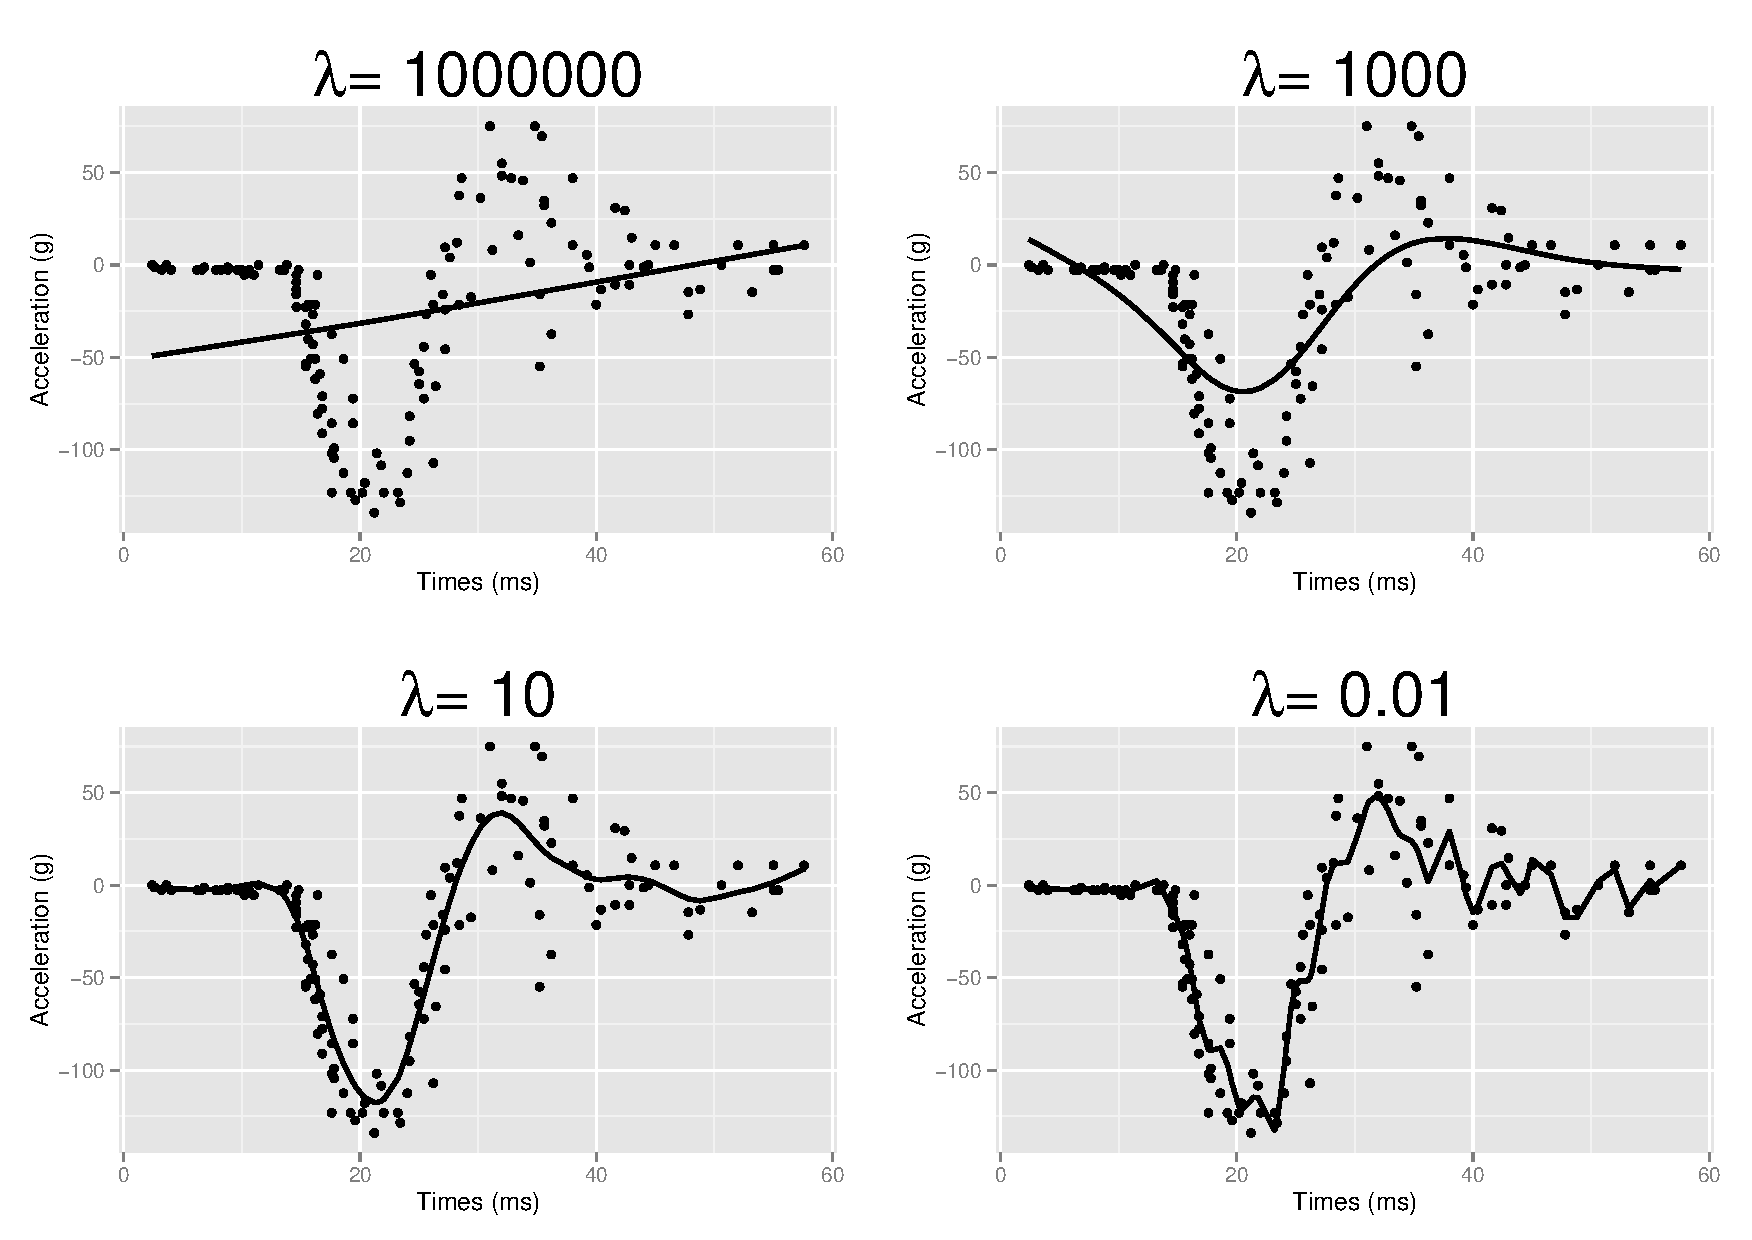
\includegraphics[height=10.5cm, width=1.05\textwidth]{Figures/LS_bspline.pdf}
%    \rule{35em}{0.5pt}
  \caption[\textit{Penalized Least Square} method using B-Splines]{\textit{Penalized Least Square} method using B-Splines on the \texttt{Motorcycle Data} with different values for the smoothing parameter}
  \label{fig:four_plots}
\end{figure}
\clearpage

%---------------------------------------------------------------------------------------
%	SECTION 4
%---------------------------------------------------------------------------------------
\FloatBarrier
\section{Model Selection}\label{section:model_selection}
The task of statistical model selection is to choose a family of distributions among a possible set of families, which is the best approximation of reality manifested in the observed data \citep{Rao2001}.

\subsection{Generalized Cross-Validation (GCV)}\label{GCV}

A measure that is popular in the spline smoothing literature is the \textit{Generalized Cross-Validation }(GCV) developed by \cite{Craven1979}. This data-driven method helps to estimate the smoothing parameter, $\lambda$, which controls the trade-off between the fit of the data and the variability in the function. It is defined to be:

\begin{align}\label{gcv}
GCV(\lambda)&=\dfrac{J^{-1}\text{RSS}}{\left[J^{-1}trace(\mathbb{I}_{J}-\bm{S_{\lambda,\phi}})\right]^{2}} \nonumber \\
            &=\left(\dfrac{J}{J-df(\lambda)}\right)\left(\dfrac{\text{RSS}}{J-df(\lambda)}\right),
\end{align}

where $df(\lambda)=trace(\mathbf{S_{\lambda,\phi}})$. \cite{olberd:ramsay} refer to the quantity in formula \eqref{gcv} as the \textit{"twice-discounted mean squared error measure''}. The minimization of GCV with respect to $\lambda$ involves trying a large set of values of $\lambda$. The GCV criterion can be expressed as:
\begin{equation}
GCV(\lambda)=\dfrac{J\times trace\left\{\bm{Y}^T_i\left[\mathbb{I}_{J}-\bm{S_{\lambda,\phi}}\right]^{-2}\bm{Y}_i\right\}}{\left\{trace\left[\mathbb{I}_{J}-\bm{S_{\lambda,\phi}}\right]\right\}^{2}},
\end{equation}

with $\mathbf{Y}_i$ be the $J \times 1$ vector of observed functional values, $\mathbf{\Phi}$ the $J \times K$ matrix of basis functions and the \textit{hat} matrix $\bm{S}_{\phi,\lambda}$ which is $J \times J$ matrix. With respect to the values of the smoothing parameter $\lambda_i$, the selected values of $\hat{\lambda}_i$ that minimize the \textit{Generalized Cross-Validation} value is the optimal value.\\
\clearpage
\subsubsection*{Numerical Example: Finding the optimal $\lambda$ using GCV}
Consider the \texttt{Motorcycle Data} smoothed using a \textit{Penalized Maximum Likelihood} method as explained in equation \eqref{penalized_likelihood}. Table~\ref{table:gcv_penls} shows the values of GCV that are derived from the $\text{log}_{10} (\lambda)$'s ranging from $-4.1$ to $-3.95$ 
\begin{table}[ht]
\caption[Minimizing the GCV yielding the optimal $\hat{\lambda}$ using \textit{Penalized Maximum Likelihood} method]{$\text{log}_{10} (\lambda)$ against GCV($\lambda$) smoothing the \texttt{Motorcycle Data}} 
\centering % used for centering table
\begin{tabular}{c c } % centered columns (4 columns)
\hline\hline %inserts double horizontal lines
&\\[-2ex]
$\text{log}_{10} (\lambda)$ & GCV($\lambda$) \\ [0.5ex] % inserts table
%heading
\hline\hline 
-4.1	&	567.6346763	\\
-4.09	&	567.6130784	\\
\textbf{-4.08}	&	\textbf{567.6067192}	\\
-4.07	&	567.616065	\\
-4.06	&	567.6415955	\\
-4.05	&	567.6838038	\\
-4.04	&	567.7431973	\\
-4.03	&	567.820297	\\
-4.02	&	567.9156388	\\
-4.01	&	568.0297766	\\
-4	&	568.1632693	\\
-3.99	&	568.3167001	\\
-3.98	&	568.4906646	\\
-3.97	&	568.6857742	\\
-3.96	&	568.902656	\\
-3.95	&	569.1419531	\\
 [0.25ex] % [1ex] adds vertical space
\hline %inserts single line
\end{tabular}
\label{table:gcv_penls} % is used to refer this table in the text
\end{table}
The optimal value for the smoothing parameteris at $\hat{\lambda} = 10^{-4.08}$. Figure~\ref{fig:gcv_plot} outputs: \textbf{(a)} the progression of the GCV-values as the $\text{log}_{10} (\lambda)$'s change with the red line showing the point where the GCV is at its lowest; \textbf{(b)} the smooth curve following the pattern of the \texttt{Motorcycle Data} using B-splines basis functions with $K = 40$ and $\hat{\lambda} = 8.317638 \times 10^{-5}$ as the smoothing parameter. Note that in this case $\hat{\sigma}^2 = 2116.593$.
\begin{figure}[th]
  %\centering
    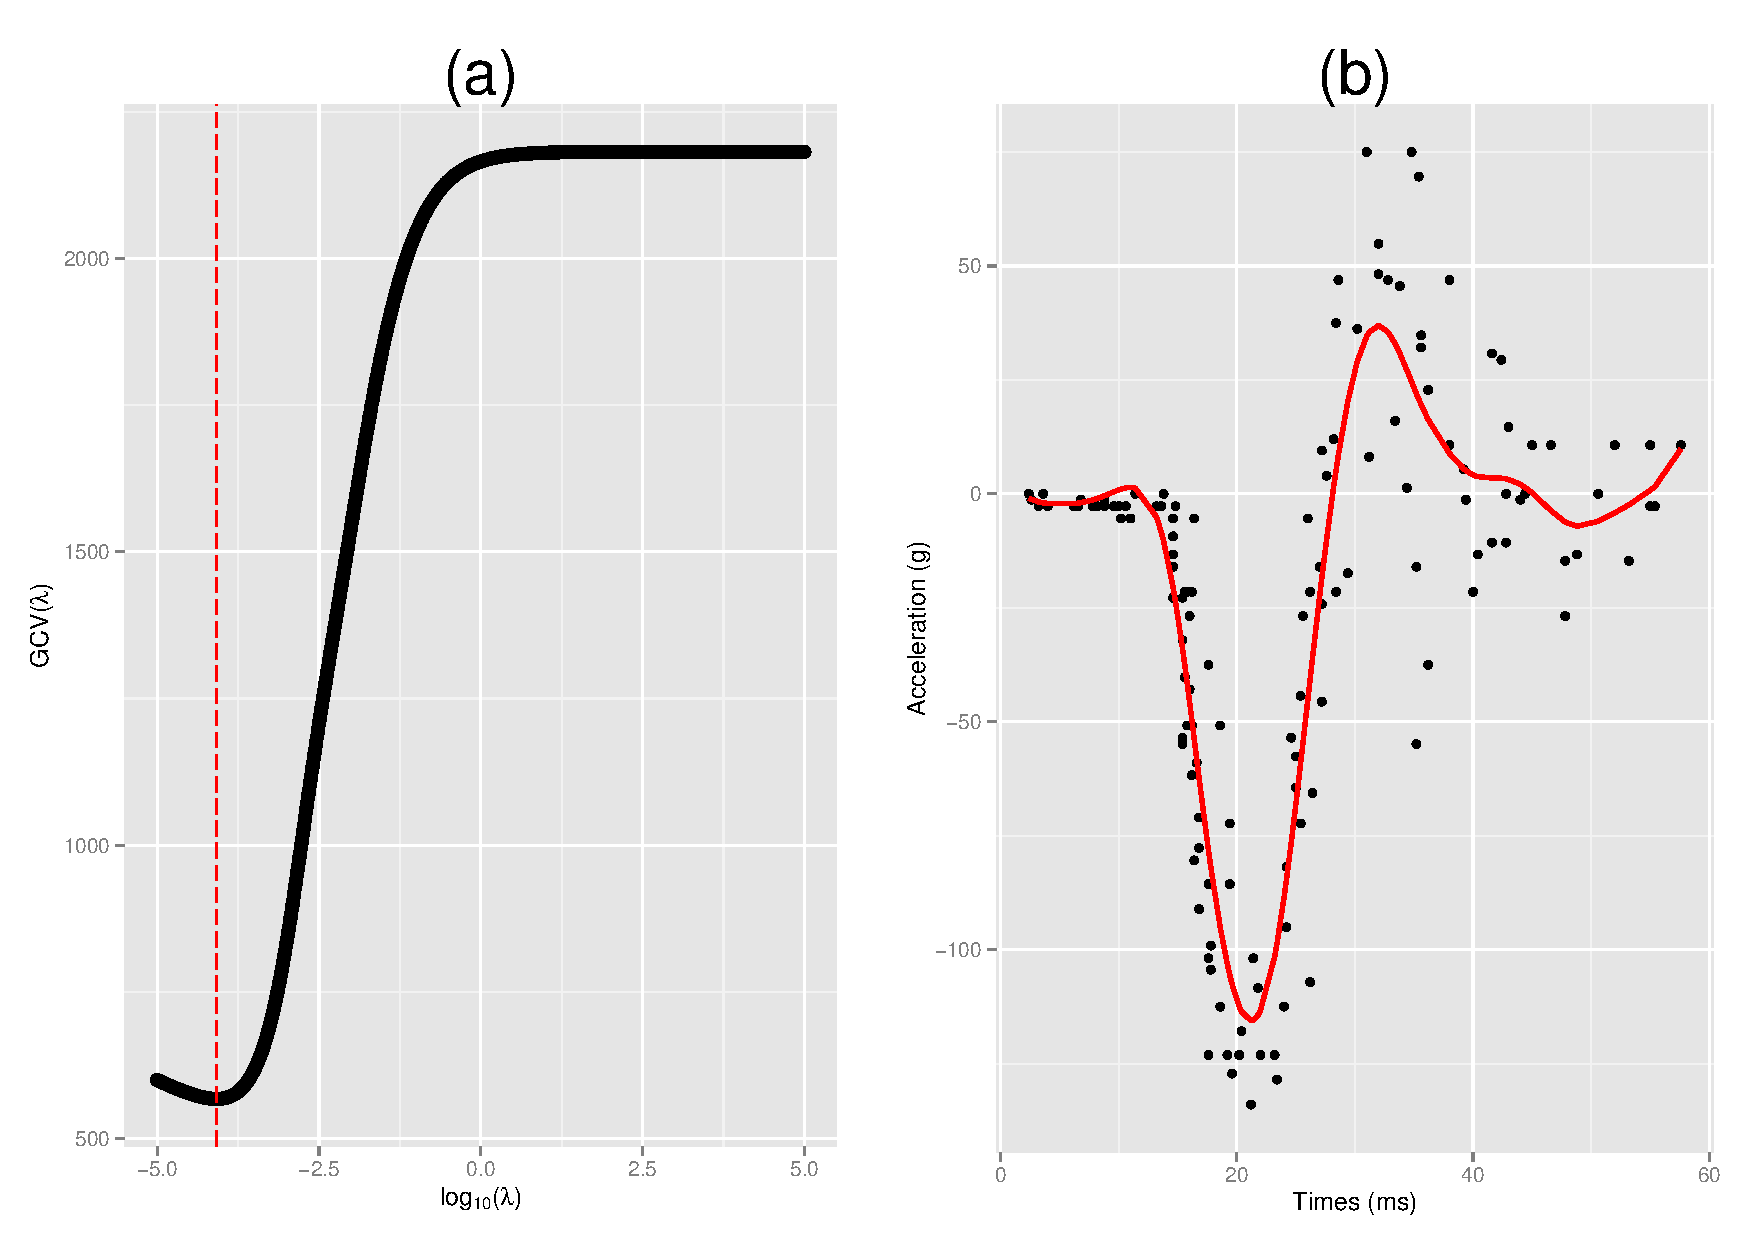
\includegraphics[height=10.5cm, width=1.1\textwidth]{Figures/Rplot_gcv.pdf}
  \caption[\textit{Penalized Maximum Likelihood} method using B-Splines]{\textbf{(a)} $\text{log}_{10} (\lambda)$ against GCV($\lambda$; \textbf{(b)} \texttt{Motorcycle Data} smoothed using \textit{B-Splines Basis} functions with $K = 40$ and GCV criterion yielding $\hat{\lambda} = 10^{-4.08}$ }
  \label{fig:gcv_plot}
\end{figure}
\clearpage

\subsection{Generalized Information Criteria (GIC)}\label{GIC}
First introduced by \cite{Konishi1996}, the GIC can be applied to evaluate statistical models constructed by various types of estimation procedures, more specifically the models estimated by maximum penalized log-likelihood procedures.

Let $G(Y)$ be the true distribution function with density $g(Y)$ that generated data, and let $\hat{G}(Y)$ be the empirical distribution function based on $J$ observations, $\bm{Y}_i = (Y_{i1},Y_{i2},\dots,Y_{iJ})^T$, drawn from $G(Y)$.  Let $\bm{\hat{\theta}}_{GIC}$ be the estimator that maximizes the penalized log-likelihood function \eqref{penalized_likelihood}. It is clear that the estimator $\bm{\hat{\theta}}_{GIC}$ is given as the solution to the following equation:

\begin{equation}
\sum_{j=1}^{J} \bm{\psi}_{GIC}(Y_{.j},\bm{\theta}) = 0,
\end{equation} 
where
\begin{equation}
\bm{\psi}_{GIC}(Y_{.j},\bm{\theta}) = \frac{\partial}{\partial \bm{\theta}} \left\{ \text{log}f(Y_{.j}|t_{.j};\bm{\theta})-\frac{\lambda_i}{2} \bm{c}^T \bm{\Omega} \bm{c} \right\}
\end{equation}
An information criterion for the model $f(Y|\bm{t};\bm{\hat{\theta}}_{GIC})$ with $\bm{\hat{\theta}}_{GIC}$ obtained by maximizing \eqref{penalized_likelihood} is given by:

\begin{equation}
\text{GIC}_{PML} = -2\sum_{j=1}^{J}\text{log}f(Y_{.j}|t_{.j};\bm{\hat{\theta}}_{GIC}) + 2\text{tr}\left\{\bm{R}(\bm{\psi}_{GIC},\hat{G})^{-1} \bm{Q}(\bm{\psi}_{GIC},\hat{G})\right\},
\end{equation}

where $\bm{R}(\bm{\psi}_{GIC},\hat{G})$ and $\bm{Q}(\bm{\psi}_{GIC},\hat{G})$ are $(K+1) \times (K+1)$ matrices given by:

\begin{align}\label{R_Q_eq}
\bm{R}(\bm{\psi}_{GIC},\hat{G})&=-\dfrac{1}{J}\sum_{j=1}^{J}\frac{\partial \bm{\psi}_{MP}(Y_{.j},\bm{\theta})^T}{\partial \bm{\theta}}\bigg|_{\bm{\hat{\theta}} = \bm{\hat{\theta}}_{GIC}}, \\
\bm{Q}(\bm{\psi}_{GIC},\hat{G})&=-\frac{1}{J}\sum_{j=1}^{J}\bm{\psi}(Y_{.j},\bm{\theta})\dfrac{\partial \text{log}f(Y_{.j}|t_{.j};\bm{\theta})}{\partial \bm{\theta}}\bigg|_{\bm{\hat{\theta}} = \bm{\hat{\theta}}_{GIC}}.
\end{align}

By setting $\text{\textit{l}}_j(\bm{\theta})=\text{log}f(Y_{ij}|t_{ij};\bm{\theta})$ (as in equation~\eqref{f_y}), its first and second partial derivatives with respect to $\bm{\theta} = \left(\bm{c}_i^T,\sigma_i^2\right)^T$ are given by:
\begin{align}
\dfrac{\partial l_j(\bm{\theta})}{\partial \sigma_i^2}&=-\dfrac{1}{2\sigma^2_i}+\dfrac{1}{2\sigma^4_i}\left\{Y_{ij}-\bm{c}_i^T\bm{\phi}(t_{ij})\right\}^2,\nonumber \\
\dfrac{\partial l_j(\bm{\theta})}{\partial \bm{c}_i}&=\dfrac{1}{\sigma_i^2}\left\{Y_{ij}-\bm{c}_i^T\bm{\phi}(t_{ij})\right\}\bm{\phi}(t_{ij}),
\end{align}

and
\begin{align}
\dfrac{\partial^2 l_j(\bm{\theta})}{\partial \sigma_i^2\partial \sigma_i^2}&=-\dfrac{1}{2\sigma^4_i}-\dfrac{1}{\sigma^6_i}\left\{Y_{ij}-\bm{c}_i^T\bm{\phi}(t_{ij})\right\}^2,\nonumber \\
\dfrac{\partial^2 l_j(\bm{\theta})}{\partial \bm{c}_i\partial \bm{c}^T_i}&=-\dfrac{1}{\sigma_i^2}\bm{\phi}(t_{ij})\bm{\phi}(t_{ij})^T, \nonumber \\
\dfrac{\partial^2 l_j(\bm{\theta})}{\partial \sigma_i^2\partial \bm{c}_i}&=-\dfrac{1}{\sigma_i^4}\left\{Y_{ij}-\bm{c}_i^T\bm{\phi}(t_{ij})\right\}\bm{\phi}(t_{ij}).
\end{align}

The matrices $\bm{R}(.)$ \& $\bm{Q}(.)$ can be derived as follows:

\begin{center}
$\dfrac{\partial \bm{\psi}_{MP}(Y_{.j},\bm{\theta})^T}{\partial \bm{\theta}}=\def\arraystretch{2}
\begin{bmatrix}
\dfrac{\partial^2 l_j(\bm{\theta})}{\partial \bm{c}_i \partial \bm{c}_i^T} - \lambda_i \bm{\Omega} & \dfrac{\partial^2 l_j(\bm{\theta})}{\partial \bm{c}_i \partial \sigma_i^2} \\
\dfrac{\partial^2 l_j(\bm{\theta})}{ \partial \sigma_i^2 \partial \bm{c}_i} & \dfrac{\partial^2 l_j(\bm{\theta})}{\partial \sigma_i^2 \partial \sigma_i^2}
\end{bmatrix}$,
\end{center}

$\bm{\psi}_{MP}(Y_{.j},\bm{\theta})\dfrac{\partial \text{log}f(Y_{.j}|t_{.j};\bm{\theta})}{\partial \bm{\theta}}$
\begin{center}
=\def\arraystretch{2}
\begin{bmatrix}
\dfrac{\partial l_j(\bm{\theta})}{\partial \bm{c}_i}\dfrac{\partial l_j(\bm{\theta})}{\partial \bm{c}_i^T} - \lambda_i \bm{\Omega}\bm{c}_i\dfrac{\partial l_j(\bm{\theta})}{\partial \bm{c}_i^T} & \dfrac{\partial l_j(\bm{\theta})}{\partial \bm{c}_i}\dfrac{\partial l_j(\bm{\theta})}{\partial \sigma_i^2} - \lambda_i \bm{\Omega}\bm{c}_i\dfrac{\partial l_j(\bm{\theta})}{\partial \sigma_i^2} \\
\dfrac{\partial l_j(\bm{\theta})}{\partial \sigma_i^2}\dfrac{\partial l_j(\bm{\theta})}{\partial \bm{c}_i^T} & \left\{\dfrac{\partial l_j(\bm{\theta})}{\partial \sigma_i^2}\right\}^2
\end{bmatrix},
\end{center}

therefore:

\begin{center}
$\bm{R}(\bm{\psi}_{GIC},\hat{G})=\dfrac{1}{J\sigma_i^2}\def\arraystretch{2}
\begin{bmatrix}
\bm{\Phi}^T\bm{\Phi}+J \lambda_i \hat{\sigma}^2_i \bm{\Omega} & \dfrac{1}{\hat{\sigma}^2_i}\bm{\Phi}^T \bm{\Lambda}_i \bm{\big{1}}_J \\
\dfrac{1}{\hat{\sigma}^2_i}\bm{\big{1}}_J^T \bm{\Lambda}_i \bm{\Phi} & \dfrac{J}{2\sigma_i^2}
\end{bmatrix}$,
\end{center}

\begin{center}
$\bm{Q}(\bm{\psi}_{GIC},\hat{G})=\dfrac{1}{J\sigma_i^2}\def\arraystretch{2}
\begin{bmatrix}
\dfrac{1}{2\sigma_i^2}\bm{\Phi}^T\bm{\Lambda}_i^2\bm{\Phi} - \lambda_i \bm{\Omega} \bm{c}_i \bm{\big{1}}_J^T \bm{\Lambda}_i \bm{\Phi} & \dfrac{1}{2\hat{\sigma}^4_i}\bm{\Phi}^T \bm{\Lambda}_i^3 \bm{\big{1}}_J - \dfrac{1}{2\hat{\sigma}^2_i}\bm{\Phi}^T \bm{\Lambda}_i \bm{\big{1}}_J \\
\dfrac{1}{2\hat{\sigma}^4_i}\bm{\big{1}}_J^T \bm{\Lambda}_i^3 \bm{\Phi}- \dfrac{1}{2\hat{\sigma}^4_i}\bm{\big{1}}_J^T \bm{\Lambda}_i \bm{\Phi} & \dfrac{1}{4\hat{\sigma}^6_i}\bm{\big{1}}_J^T \bm{\Lambda}_i^4 \bm{\big{1}}_J-\dfrac{J}{4\sigma_i^2}
\end{bmatrix}$,
\end{center}
where $\bm{\big{1}}_J = (1,1,\dots,1)^T$ is a $J$-dimensional vector of 1's, and $\bm{\Lambda}$ is a $J \times J$ diagonal matrix defined by

\begin{equation*}
\bm{\Lambda}_i = \text{diag} \left[Y_{i1} - \bm{\hat{c}}_i^T\bm{\phi}(t_{i1}),Y_{i2} - \bm{\hat{c}}_i^T\bm{\phi}(t_{i2}),\dots,Y_{iJ} - \bm{\hat{c}}^T_i\bm{\phi}(t_{iJ})\right]
\end{equation*}

\subsubsection*{Numerical Example: Finding the optimal $\lambda$ using GIC}
Consider the \texttt{Motorcycle Data} smoothed using the \textit{Penalized Maximum Likelihood} method as explained in equation \eqref{penalized_likelihood}. Table~\ref{table:gic_penml} shows the values of GIC that are derived from the $\text{log}_{10} (\lambda)$'s ranging from $-4.3$ to $-4.1$ 
\begin{table}[ht]
\caption[Minimizing the GIC yields to the optimal $\hat{\lambda}$ using \textit{Penalized Maximum Likelihood} method]{$\text{log}_{10} (\lambda)$ against GIC($\lambda$) smoothing the \texttt{Motorcycle Data}} 
\centering % used for centering table
\begin{tabular}{c c } % centered columns (4 columns)
\hline\hline %inserts double horizontal lines
&\\[-2ex]
$\text{log}_{10} (\lambda)$ & GIC($\lambda$) \\ [0.5ex] % inserts table
%heading
\hline\hline 
-4.3	&	1216.693	\\
-4.29	&	1216.679	\\
-4.28	&	1216.666	\\
-4.27	&	1216.655	\\
-4.26	&	1216.646	\\
-4.25	&	1216.639	\\
-4.24	&	1216.633	\\
-4.23	&	1216.630	\\
\textbf{-4.22}	&	\textbf{1216.629}	\\
-4.21	&	1216.630	\\
-4.2	&	1216.633	\\
-4.19	&	1216.638	\\
-4.18	&	1216.646	\\
-4.17	&	1216.656	\\
-4.16	&	1216.669	\\
-4.15	&	1216.684	\\
-4.14	&	1216.702	\\
-4.13	&	1216.723	\\
 [0.25ex] % [1ex] adds vertical space
\hline %inserts single line
\end{tabular}
\label{table:gic_penml} % is used to refer this table in the text
\end{table}
The optimal value for the smoothing parameter is at $\hat{\lambda} = 10^{-4.22}$. Figure~\ref{fig:gic_plot} outputs: \textbf{(a)} the progression of the GIC-values as the $\text{log}_{10} (\lambda)$'s change with the red line showing the point where the GIC is at its lowest; \textbf{(b)} the smooth curve following the pattern of the \texttt{Motorcycle Data} using \textit{B-Splines Basis} functions with $K = 40$ and $\hat{\lambda} = 6.025596 \times 10^{-5}$ as the smoothing parameter. It is important to note that $\hat{\sigma}^2 = 462.5911$.

\begin{figure}[th]
  %\centering
    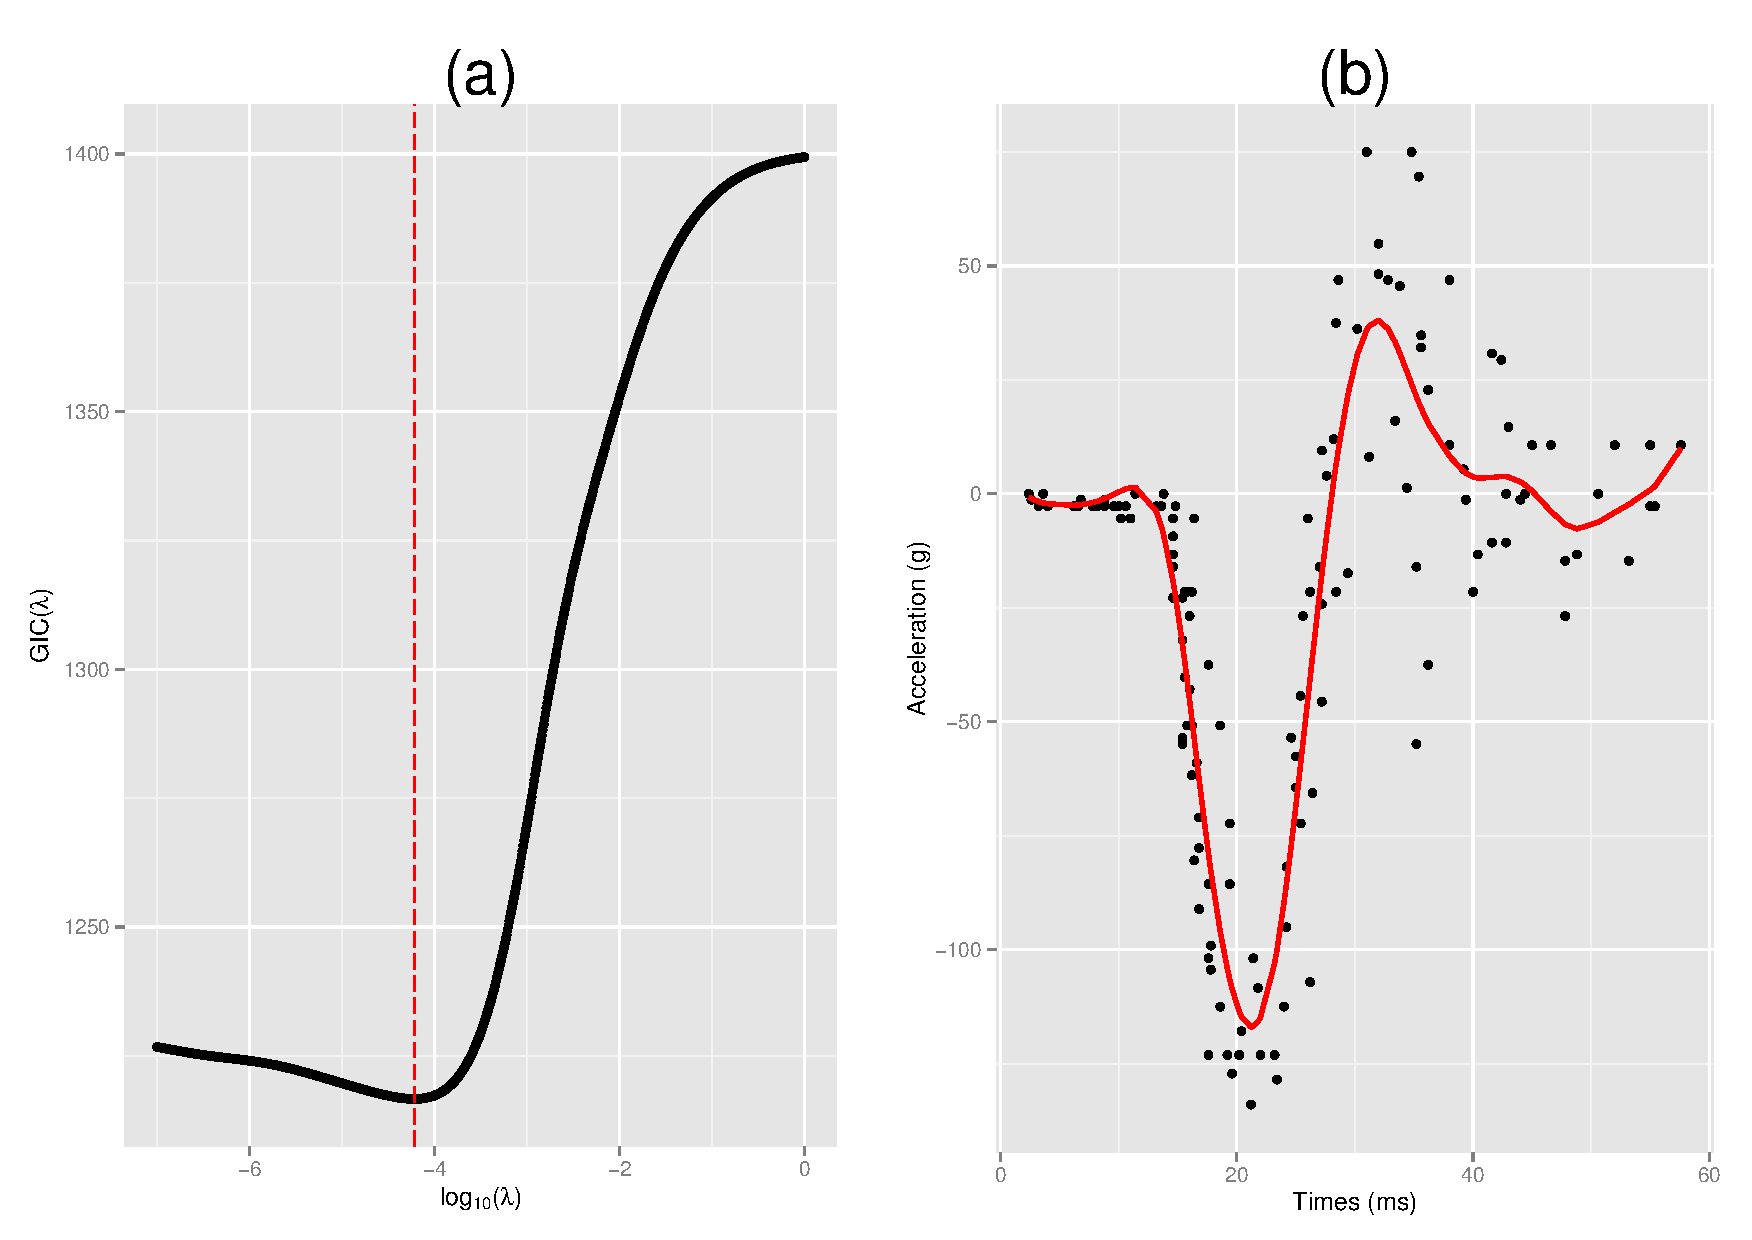
\includegraphics[height=10.5cm, width=1.1\textwidth]{Figures/Rplot_gic.pdf}
  \caption[\textit{Penalized Maximum Likelihood} method evaluated using GIC]{\textbf{(a)} $\text{log}_{10} (\lambda)$ against GIC($\lambda$); \textbf{(b)} \texttt{Motorcycle Data} smoothed using\textit{B-Splines Basis} functions with $K = 40$ and GIC criterion yielding $\hat{\lambda} = 10^{-4.22}\text{ }\&\text{ }\hat{\sigma}^2 = 462.5911$ }
  \label{fig:gic_plot}
\end{figure}
%The minimization of \textit{GIC} with respect to the model parameters will involve trying to inspect a large number of values where at least one of these values will be the optimal value.

\subsection{Modified Akaike Information Criteria (mAIC)}\label{mAIC}
The Akaike's information criteria (1973) was derived as an estimator of the \cite{kullback1951} information from the predictive point of view. It is given by:

\begin{equation}\label{aic}
-2 l(\bm{Y}_i|\bm{\hat{\theta}}_{ML}) + 2(\text{number of parameters})
\end{equation} 

where $l(\bm{\hat{\theta}}_{ML})$ is the log-likelihood of a model estimated by the \textit{Maximum Likelihood} and the ``number of parameters'' is a measure of complexity of the model. However, in nonlinear modelling, the ``number of parameters'' is not an appropriate measure of model complexity since it may depend on both the regularization term and the observed data. \cite{Fujikoshi1997} considered using the trace \textit{smoother operator} (see equations \eqref{project_op1} \& \eqref{project_op2}) as an approximation to the effective ``number of parameters''. By replacing the last term in \eqref{aic} by $\text{tr }(S_{\lambda_i})$, the \textit{mAIC} is given by:

\begin{equation}
\text{mAIC} = J \text{ log}(2 \pi \hat{\sigma}_i^2) + J + 2\text{ tr}(S_{\lambda_i})
\end{equation}

\subsubsection*{Numerical Example: Finding the optimal $\lambda$ using mAIC}
The \texttt{Motorcycle Data} is smoothed using the \textit{penalized maximum likelihood}. Table~\ref{table:maic_penml} is showing the values of mAIC that are derived from the $\text{log}_{10} (\lambda)$'s ranging from $-4.2$ to $-4.05$. 
\begin{table}[ht]
\caption[Minimizing the mAIC yields to the optimal $\hat{\lambda}$ using \textit{Penalized Maximum Likelihood} method]{$\text{log}_{10} (\lambda)$ against mAIC($\lambda$) smoothing the \texttt{Motorcycle Data}} 
\centering % used for centering table
\begin{tabular}{c c } % centered columns (4 columns)
\hline\hline %inserts double horizontal lines
&\\[-2ex]
$\text{log}_{10} (\lambda)$ & mAIC($\lambda$) \\ [0.5ex] % inserts table
%heading
\hline\hline 
-4.2	&	1216.633	\\
-4.19	&	1216.638	\\
-4.18	&	1216.646	\\
-4.17	&	1216.656	\\
-4.16	&	1216.669	\\
-4.15	&	1216.684	\\
-4.14	&	1216.702	\\
-4.13	&	1216.723	\\
\textbf{-4.12}	&	\textbf{1216.747}	\\
-4.11	&	1216.774	\\
-4.1	&	1216.803	\\
-4.09	&	1216.836	\\
-4.08	&	1216.873	\\
-4.07	&	1216.913	\\
-4.06	&	1216.956	\\
-4.05	&	1217.003	\\
 [0.25ex] % [1ex] adds vertical space
\hline %inserts single line
\end{tabular}
\label{table:maic_penml} % is used to refer this table in the text
\end{table}
The optimal value for the smoothing parameter is at $\hat{\lambda} = 10^{-4.12}$. Figure~\ref{fig:maic_plot} outputs: \textbf{(a)} the progression of the mAIC-values as the $\text{log}_{10} (\lambda)$'s change with the red line showing the point where the mAIC is at its lowest; \textbf{(b)} the smooth curve following the pattern of the \texttt{Motorcycle Data} using \textit{B-Splines Basis} functions with $K = 40$ and $\hat{\lambda} = 7.585776 \times 10^{-5}$ as the smoothing parameter. Note that$\hat{\sigma}^2 = 466.3463$

\begin{figure}[th]
  %\centering
    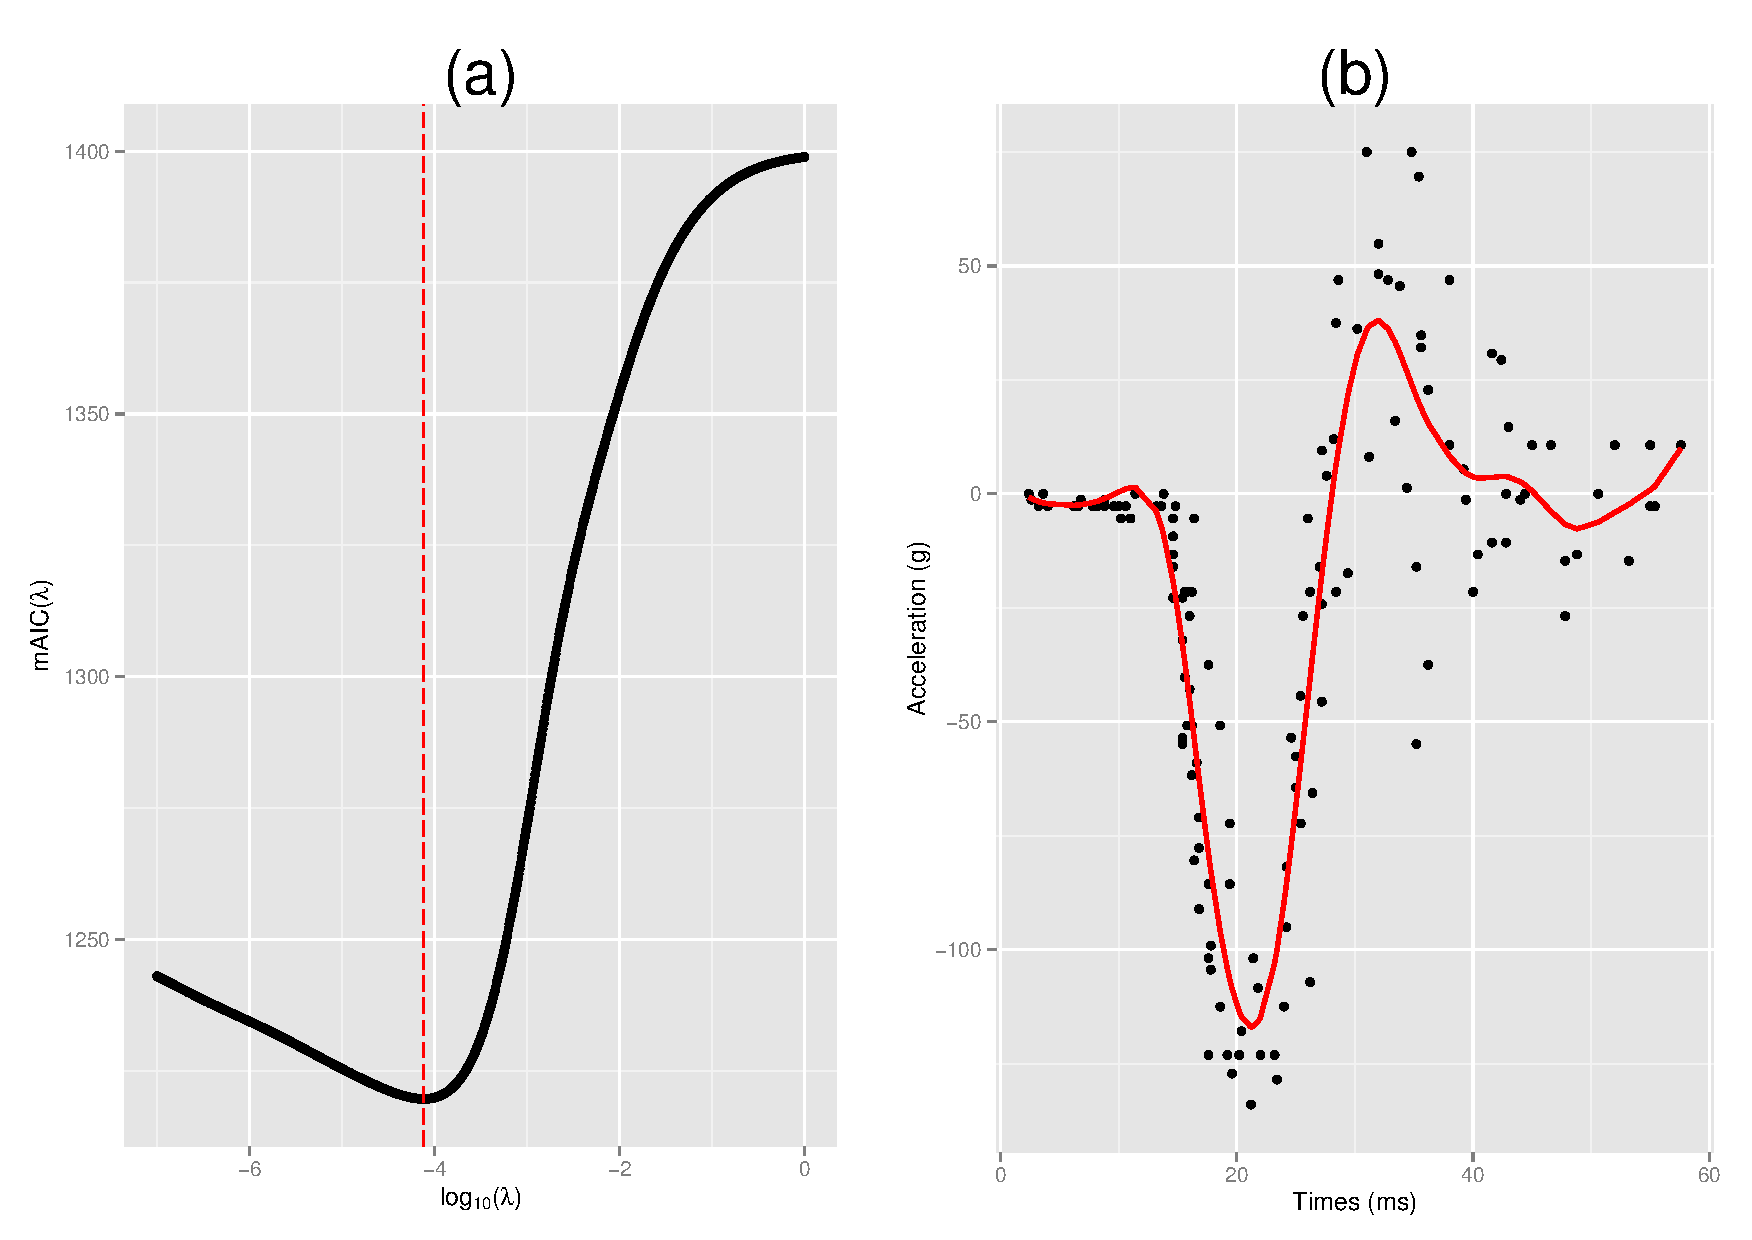
\includegraphics[height=10.5cm, width=1.1\textwidth]{Figures/Rplot_maic.pdf}
  \caption[\textit{Penalized Maximum Likelihood} method evaluated using mAIC]{\textbf{(a)} $\text{log}_{10} (\lambda)$ against mAIC($\lambda$); \textbf{(b)} \texttt{Motorcycle Data} smoothed using B-splines basis functions with $K = 40$ and mAIC criterion yielding $\hat{\lambda} = 10^{-4.12}\text{ }\&\text{ }\hat{\sigma}^2 = 466.3463$ }
  \label{fig:maic_plot}
\end{figure}
\clearpage

\subsection{Generalized Bayesian Information Criteria (GBIC)}\label{GBIC} 
Derived from the well known \textit{Bayesian Information Criteria} (BIC), it is a model selection criterion used to evaluate models fitted by the \textit{Penalized Maximum Likelihood} method or the method of \textit{Regularization}. \cite{Konishi2004} derived this criterion in order to estimate the smoothing parameters as well as other parameters such as the number of basis functions.\\
Suppose that the suitable model is constructed by maximizing equation~\eqref{penalized_likelihood} yielding the maximum likelihood estimators for $\bm{c}_i$ and $\sigma^2_i$ (see equation~\ref{solution_eqpen}). Considering $\beta_i = \lambda_i \sigma^2_i$ and subsituting back in equation~\eqref{solution_eqpen}, the \textit{Generalized Bayesian Information Criteria} is given by: 
\begin{eqnarray}
\text{GBIC }&=&(J+K-1)\text{ log}\hat{\sigma}^2_i + J \beta_i\hat{\bm{c}}^T_i \bm{\Omega} \hat{\bm{c}}_i /\hat{\sigma}^2_i + J +(J-3)\text{ log}(2\pi) + 3\text{ log}J \nonumber\\ 
&& + \text{ log} |\bm{Q}_{\beta_i}^{(G)} (\hat{\bm{c}}^T_i,\hat{\sigma}^2_i)| - \text{ log}|\bm{\Omega}|_{+} - (K-1)\text{ log} \beta_i
\end{eqnarray}
where $|\bm{\Omega}| _{+}$ denotes the product of nonzero eigenvalues of $\bm{\Omega}$ and
\begin{center}
$\bm{Q}_{\beta_i}^{(G)} (\hat{\bm{c}}^T_i,\hat{\sigma}^2_i)=\dfrac{1}{J\sigma_i^2}\def\arraystretch{2}
\begin{bmatrix}
\bm{\Phi}^T\bm{\Phi} + J \beta_i \bm{\Omega} & \bm{\Phi}^T \bm{e} / \hat{\sigma}^2_i \\
\bm{e}^T \bm{\Phi} / \hat{\sigma}^2_i & \dfrac{J}{2\sigma_i^2}
\end{bmatrix}$.
\end{center}
Note that $\bm{e}$ is a $J$-dimensional vector given by
\begin{equation*}
\bm{e} = \left[Y_{i1} - \bm{\hat{c}}_i^T\bm{\phi}(t_{i1}),Y_{i2} - \bm{\hat{c}}_i^T\bm{\phi}(t_{i2}),\dots,Y_{iJ} - \bm{\hat{c}}^T_i\bm{\phi}(t_{iJ})\right]^T.
\end{equation*}
For a more extensive derivation of the above result, consult the journal article written by \cite{Konishi1996}.

\subsubsection*{Numerical Example: Finding the optimal $\lambda$ using GBIC}
The \texttt{Motorcycle Data} is smoothed using the \textit{Penalized Maximum Likelihood}. Table~\ref{table:gbic_penml} is showing the values of GBIC that are derived from the $\text{log}_{10} (\lambda)$'s ranging from $-4.3$ to $-4.15$ 
\begin{table}[ht]
\caption[Minimizing the GBIC yields to the optimal $\hat{\lambda}$ using \textit{Penalized Maximum Likelihood} method]{$\text{log}_{10} (\lambda)$ against GBIC($\lambda$) smoothing the \texttt{Motorcycle Data}} 
\centering % used for centering table
\begin{tabular}{c c } % centered columns (4 columns)
\hline\hline %inserts double horizontal lines
&\\[-2ex]
$\text{log}_{10} (\lambda)$ & GBIC($\lambda$) \\ [0.5ex] % inserts table
%heading
\hline\hline 
-4.3	&	1258.324	\\
-4.29	&	1258.288	\\
-4.28	&	1258.257	\\
-4.27	&	1258.232	\\
-4.26	&	1258.213	\\
-4.25	&	1258.200	\\
-4.24	&	1258.193	\\
\textbf{-4.23}	&	\textbf{1258.192}	\\
-4.22	&	1258.196	\\
-4.21	&	1258.208	\\
-4.2	&	1258.225	\\
-4.19	&	1258.249	\\
-4.18	&	1258.279	\\
-4.17	&	1258.315	\\
-4.16	&	1258.358	\\
-4.15	&	1258.408	\\
 [0.25ex] % [1ex] adds vertical space
\hline %inserts single line
\end{tabular}
\label{table:gbic_penml} % is used to refer this table in the text
\end{table}
The optimal value for the smoothing parameter is at $\hat{\lambda} = 10^{-4.23}$. Figure~\ref{fig:gbic_plot} outputs: \textbf{(a)} the progression of the mAIC-values as the $\text{log}_{10} (\lambda)$'s change with the red line showing the point where the mAIC is at its lowest; \textbf{(b)} the smooth curve following the pattern of the \texttt{Motorcycle Data} using \textit{B-Splines Basis} functions with $K = 40$ and $\hat{\lambda} = 5.888437 \times 10^{-5}$ as the smoothing parameter. Note that $\hat{\sigma}^2 = 462.2833$

\begin{figure}[th]
  %\centering
    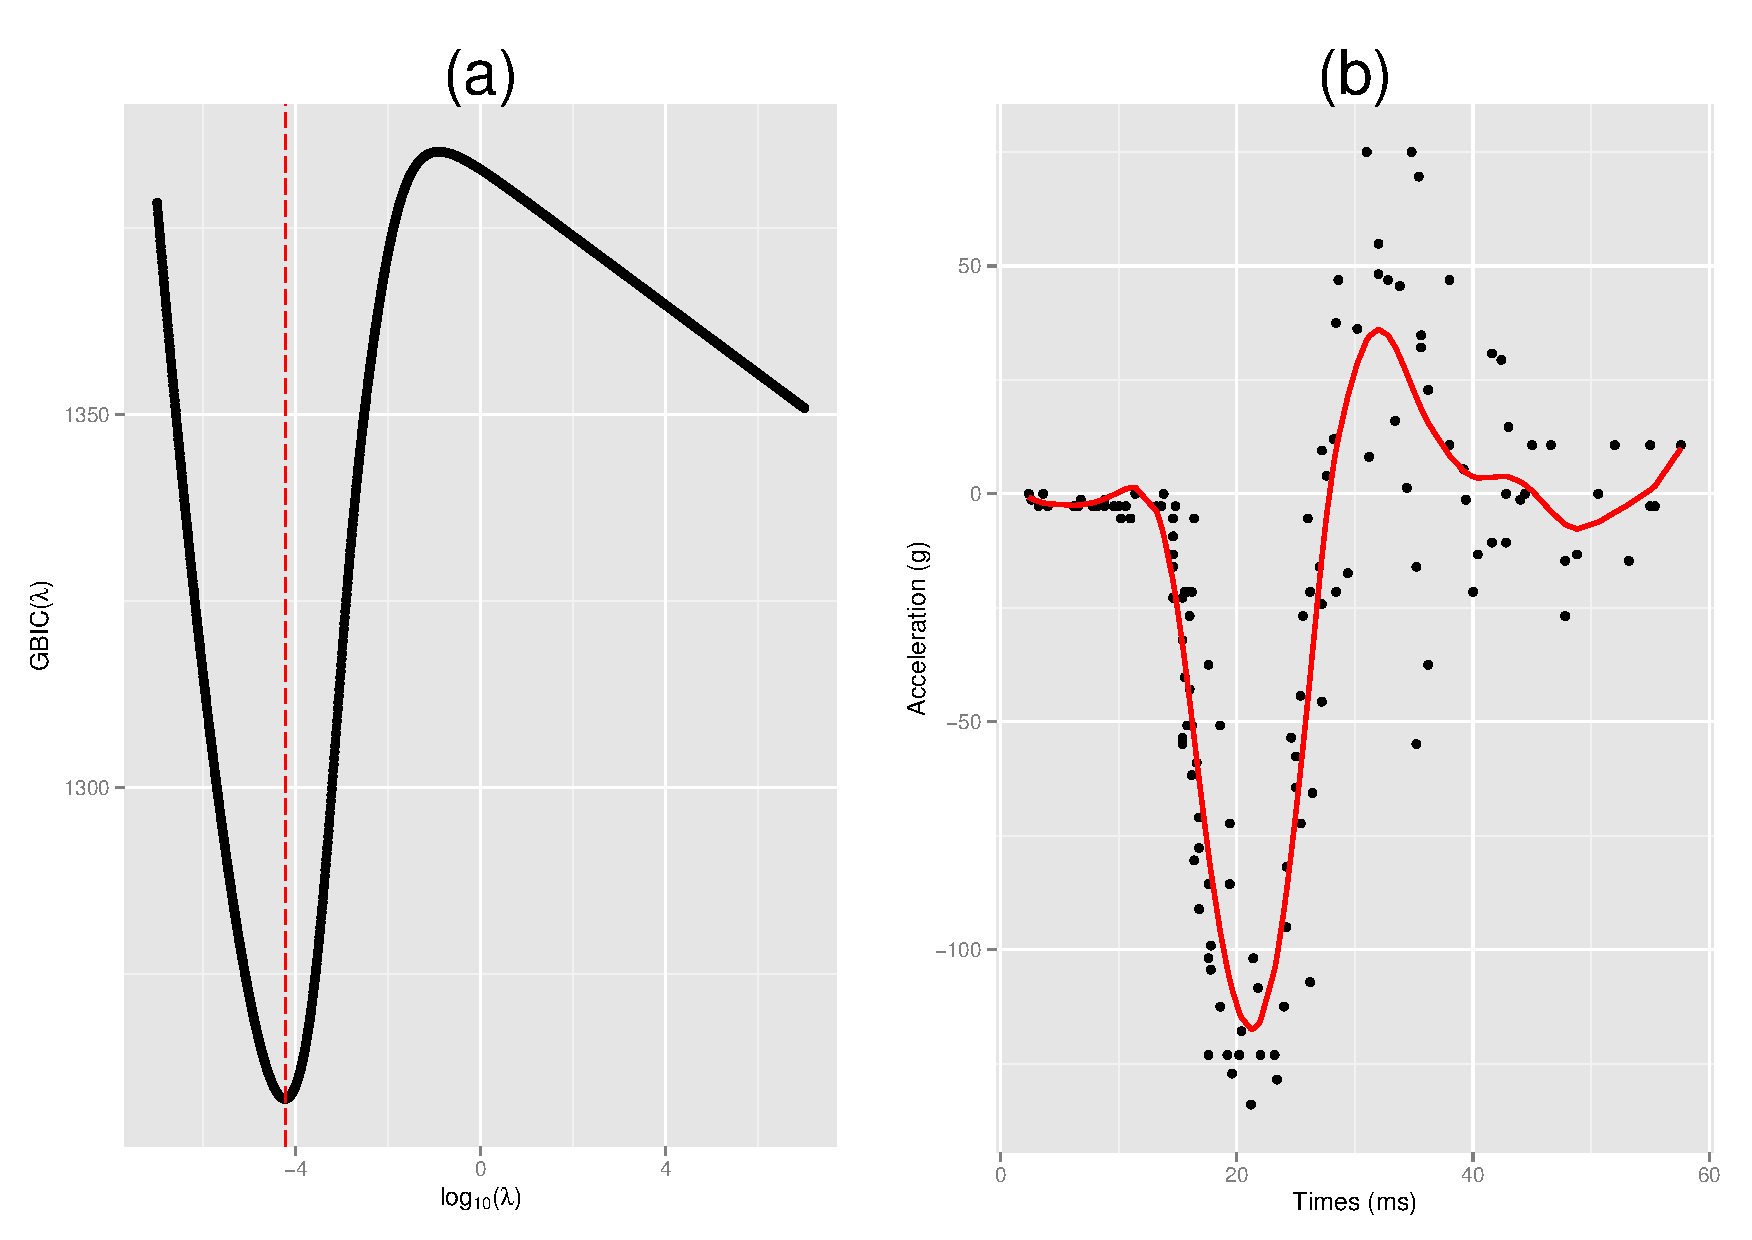
\includegraphics[height=10.5cm, width=1.1\textwidth]{Figures/Rplot_gbic.pdf}
  \caption[\textit{Penalized Maximum Likelihood} method evaluated using GBIC]{\textbf{(a)} $\text{log}_{10} (\lambda)$ against GBIC($\lambda$); \textbf{(b)} \texttt{Motorcycle Data} smoothed using \textit{B-splines} basis functions with $K = 40$ and GBIC criterion yielding $\hat{\lambda} = 10^{-4.23}\text{ }\&\text{ }\hat{\sigma}^2 = 462.2833$ }
  \label{fig:gbic_plot}
\end{figure}
\clearpage

Although the \textit{Generalized Cross-Validation} criterion is widely used for the regularization parameter selection, the computational time is very large and high variability and tendency to undersmooth are not negligible in the analysis of Functional Data \citep{Matsui2009}. Table~\ref{table:summary1} illustrates that argument with a high value for the GCV Mean Square Errors (MSE) as well as its estimated $\hat{\sigma}_{GCV}^2$; it is important to point out that the number of basis functions is the same for all model criteria. 

\begin{table}[ht]
\caption[Summary of the model selection applied on the \texttt{Motorcycle Data} with $K = 40$]{Summary of the model selection applied on the \texttt{Motorcycle Data} smoothed using B-splines basis functions with $K = 40$}
\centering % used for centering table
\begin{tabular}{c @{\hspace{0.2cm}\vrule width 2pt\hspace{0.2cm}} c c c } % centered columns (4 columns)
\hline %inserts double horizontal lines
\multicolumn{1}{c}{} & & &  \\[-2ex]
 \multicolumn{1}{c}{}& $\text{log}_{10} (\hat{\lambda})$ & $\hat{\sigma}^2$ & MSE \\ [0.5ex] % inserts table
%heading
\noalign{\hrule height 1pt} 
GCV &	-4.08 & \textbf{2116.593}	&	\textbf{468.1117}	\\
GIC &	-4.22 & 462.5911	&	462.5911	\\
mAIC &	-4.12 & 466.3463	&	466.3463	\\
GBIC &	-4.23 & 462.2833	&	462.2833	\\
 [0.25ex] % [1ex] adds vertical space
\hline  %inserts single line
\end{tabular}
\label{table:summary1} % is used to refer this table in the text
\end{table}

\subsection{The optimal number \textit{K} of Basis Functions}
Choosing the optimal number $K$ of basis functions is an important task when converting the discrete observations into Functional Data. The larger $K$ the better the fit to the data, but at the same time the risk of fitting noise or variation that should not be ignored. On the other hand, if $K$ is too small, some important aspects of the smooth function might be disregarded when trying to estimate the function \citep{olberd:ramsay}. One of the main reasons for smoothing is to reduce the influence of noise as well as to capture meaningful regularities on the estimates. The idea of the penalization is to rather overfit the data and then penalize to obtain a bias-variance trade-off. The methods for model selection (mentioned above) may offer some guidance in the choice of the optimal $K$, however for each value of the number of basis functions there is an optimal value for $\hat{\lambda}$ \& $\hat{\sigma}^2$. 
%---------------------------------------------------------------------------------------
%	SECTION 5
%---------------------------------------------------------------------------------------
\clearpage
\section{Functional Descriptive Statistics}
One of the most important parts in data analysis is the exploratory part: Estimating means and standard deviations. Because the functional nature of the data, the associated descriptive statistics are therefore functional.

\subsection{Mean \& Variance functions}
Estimating the \textit{Mean Function} based on discretely sampled noisy observations is one of the most basic problems in Functional Data Analysis. The \textit{Mean Function} is a simple analogue of the classical mean for univariate data. It can be calculated by averaging the functions point-wise across the replications, since Functional Data Analysis sees each curve as a distinct datum itself. The mean function is defined as $\mathbf{\nu}_{\mathcal{X}}(t)=\mathbb{E}(X(t)),\text{ }\forall t \in \mathcal{T}$. The sample mean curve is: 

\begin{equation} \label{eq:functmean}
\bar{X}(t)=\frac{1}{N}(X_{1}(t)+\dots+X_{N}(t)),\text{ }\forall t \in \mathcal{T} 
\end{equation}

where \textit{N} is the number of curves or replications and $X_{i}(t)$ is the \textit{i-th} function evaluated at time \textit{t}. Below is a plot illustrating the concept of \textit{Functional Mean} applied on the \texttt{Canadian Weather} dataset from \cite{olberd:ramsay}. The \textit{Functional Mean} is calculated for five weather stations namely \textit{St.Johns, Halifax, Sydney, Yarmouth \& Charlottville} represented using a \textit{Fourier Basis} expansion with $K = 65$:
\begin{figure}[h]
  \centering
    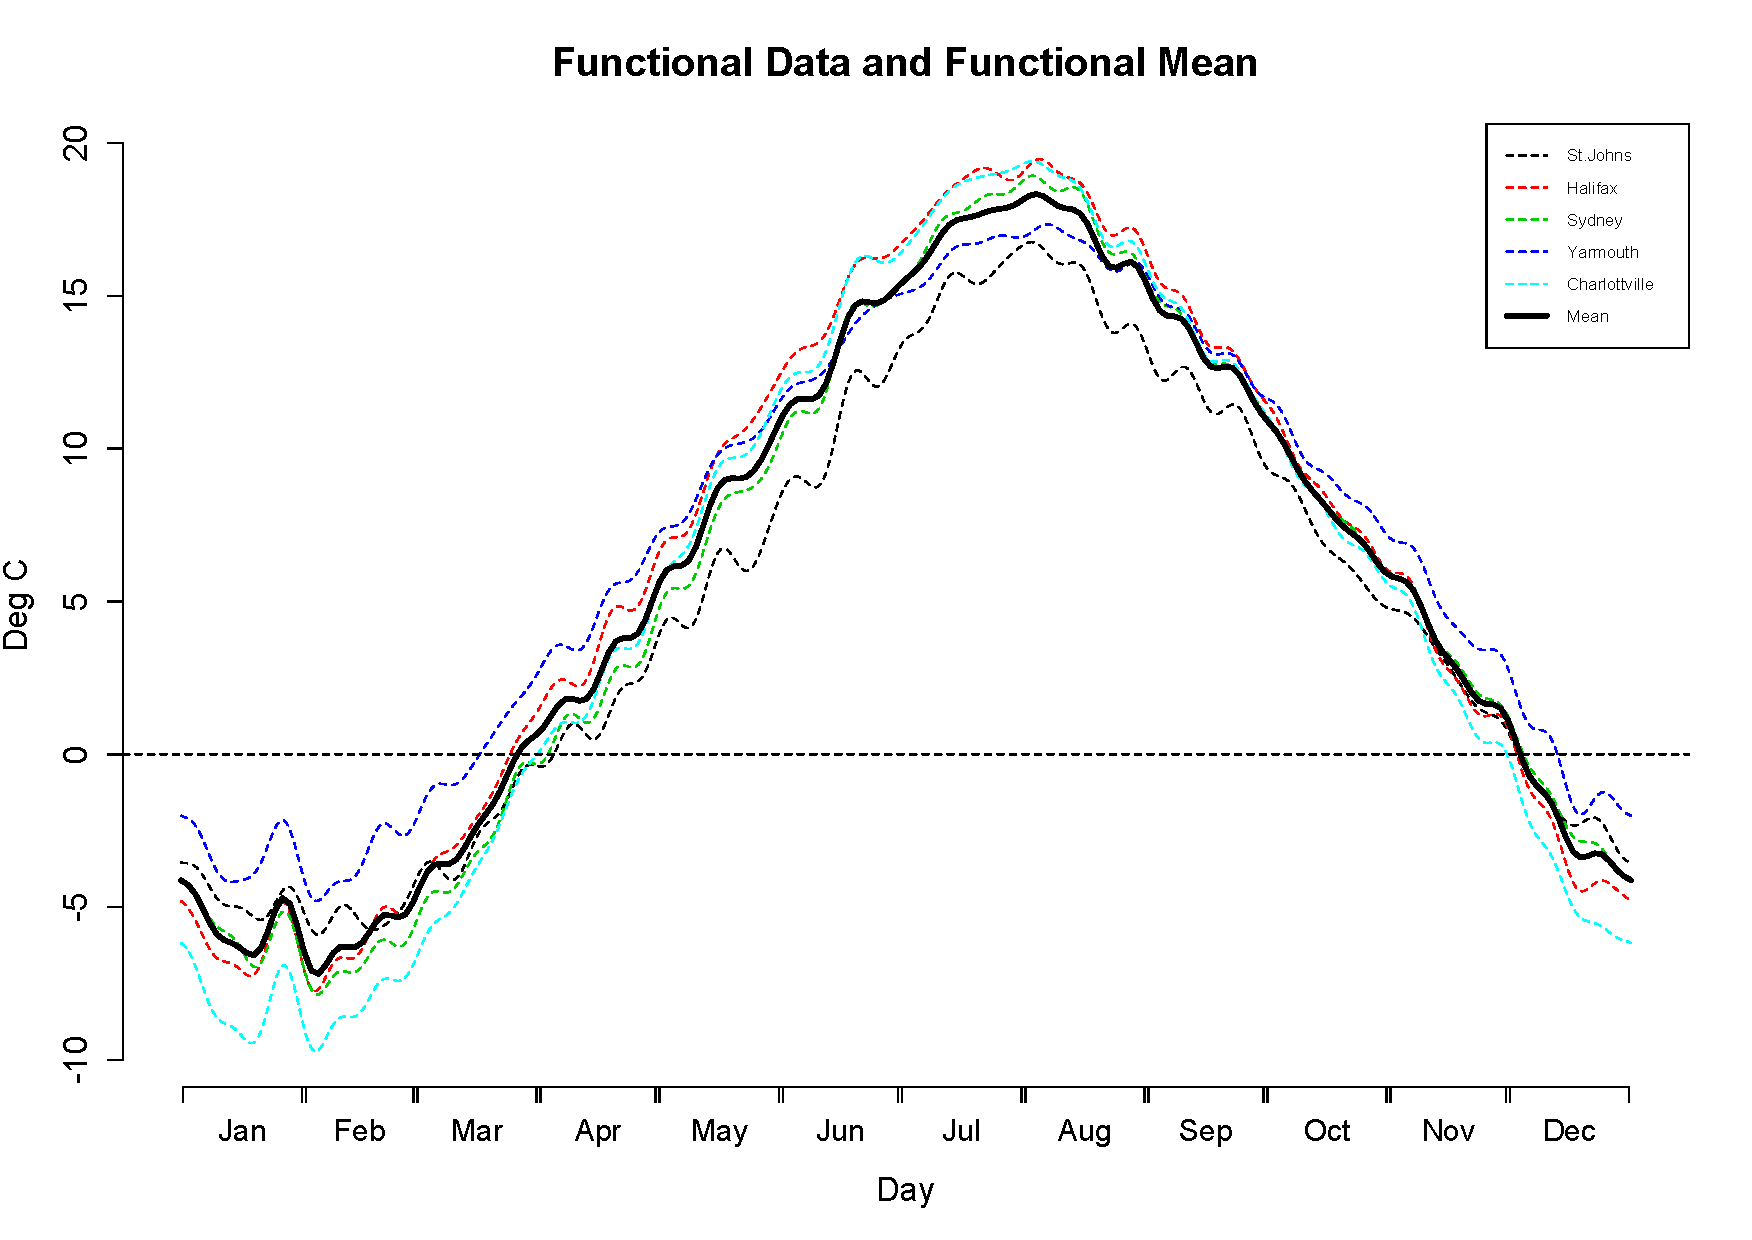
\includegraphics[height=7cm, width=1\textwidth]{Figures/functionalmean1.pdf}
%    \rule{35em}{0.5pt}
  \caption[\textit{Functional Mean} applied on Canadian Weather dataset]{Canadian Weather data: Mean Curve \footnote{I need to introduce a legend on the plot.}.}
  \label{fig:meancurve}
\end{figure}

Likewise, the estimation of the \textit{Functional Variance} is very similar to the classical variance for univariate data. It is defined as $\mathbf{\sigma}^{2}_{\mathcal{X}}(t)=\mathbb{E}\left[(X(t)-\nu_{\mathcal{X}}(t))^{2}\right],\text{ }\forall t \in \mathcal{T}$.  The sample variance curve is:
\begin{equation}
\textbf{var}_{\mathcal{X}}(t)=\dfrac{1}{N}\sum\limits_{i=1}^{N}\left[X_{i}(t)-\bar{X}(t)\right]^{2}
\end{equation}
and the standard deviation function is the square root of the variance function.

\subsection{Covariance and Correlation functions}
The \textit{covariance function} summarizes the dependence of records across different argument values. We define $\Gamma_{\mathcal{X}}$ to be the covariance function

\begin{equation*}
\Gamma_{\mathcal{X}}(t_{1},t_{2})=\mathbb{E}\left[(X(t_{1})-\nu_{\mathcal{X}}(t_{1}))(X(t_{2})-\nu_{\mathcal{X}}(t_{2}))\right], \text{ } \forall t_{1},t_{2} \in \mathcal{T},
\end{equation*}

and $\hat{\Gamma}$ to be the sample covariance function

\begin{equation}\label{covar}
\hat{\Gamma}(t_{1},t_{2})=\frac{1}{N}\sum\limits_{i=1}^{N}\{X_{i}(t_{1})-\bar{X}(t_{1})\}\{X_{i}(t_{2})-\bar{X}(t_{2})\},  \text{ } \forall t_{1},t_{2} \in \mathcal{T}.
\end{equation}

The associated \textit{correlation function} is

\begin{equation}
\textbf{corr}_{\mathcal{X}}(t_{1},t_{2})=\frac{\hat{\Gamma}_{\mathcal{X}}(t_{1},t_{2})}{\sqrt{\textbf{var}_{\mathcal{X}}(t_{1})\textbf{var}_{\mathcal{X}}(t_{2})}}
\end{equation}

%Figure \ref{fig:corrcurve} gives us a symmetrical three-dimensional correlation surface where the diagonal ridge running from the lower left to the upper right is exactly one and the parts on each side of the ridge representing the correlations of temperatures at every two time combinations of the year. In functional data framework, we can calculate the correlation of values at every two points along the curves.
%%\vskip
%\begin{figure}[ht]
%  \centering
%    \includegraphics[height=8.9cm, width=1\textwidth]{Pictures/ex-weather-bfig4.png}
%%    \rule{35em}{0.5pt}
%  \caption[Temperature Correlation Function]{Canadian Weather data: Temperature Correlation Function \footnote{I need to introduce a legend on the plot.}.}
%  \label{fig:corrcurve}
%\end{figure}
\clearpage


%---------------------------------------------------------------------------------------
%	SECTION 5
%---------------------------------------------------------------------------------------
\section{Parallel Computing using \tt{R}}
Dealing with large data sets has become common practice when working with Functional Data. Statisticians usually find the need to perform some operations repeatedly for model selection or simply to execute functions with multiple arguments.
Repeated executions can be done manually, but it becomes quite tedious to execute repeated operations even with the use of command line editing (Leach, 2014). Nowadays, all computers are equipped with multicore processors which allow splitting tasks across a number of cores for execution and therefore reducing computation time.

\subsection{Parallel Backends}
 Running codes in parallel is not a default feature of \texttt{R}, so executing parallelism requires to first make the desired number of cores available to \texttt{R} by registring a \textit{parallel backend} which effectively creates a cluster to which computations can be sent to. Several packages have been developped to handle this process:
 
 \begin{itemize}
 \item \textbf{doMC} \citep{doMC}
 \item \textbf{doSNOW} \citep{doSNOW}
 \item \textbf{doParallel} \citep{doParallel}
 \end{itemize}
Creating a cluster is done using the following lines of codes:
\vskip

\begin{lstlisting}
suppressPackageStartupMessages(library(doParallel))
detectCores() # how many cores are available
workers <- makeCluster(6) # create a cluster with 6 cores
registerDoParallel(workers) # register cluster
getDoParWorkers() # Number of cores that will be used
\end{lstlisting}


\subsection{Using \texttt{foreach}}\label{foreach}
The \texttt{foreach} package provides a new looping construct for processing \texttt{R} codes repeatedly \citep{foreach}. It supports \textit{parallel execution}, in other words it can process replicated operations on multiple cores on the computer or on multiple nodes of a cluster.\\
For illustrations purpose, consider the temperature data from the \texttt{Aemet} dataset in \texttt{R}. Given a set of values for $K$ ranging from 5 to 360, the \textit{Generalized Cross-Validation} is computed for each $K$ and the time taken to process the \texttt{R}-script with and without \texttt{foreach} is recorded.
\subsubsection*{Without \texttt{foreach}}

 \begin{lstlisting}
  #### Temperature
  data(aemet,package = "fda.usc")
  tt <- aemet$temp$argvals
  temp <- aemet$temp$data
  cent.temp <- apply(X = temp,MARGIN = 2,FUN = scale, scale=FALSE)
  m <- seq(5,360)
  temp_gcv <- rep(0,length(m))
  count <- 0
  ptime <- system.time(for (i in m){
 +   count <- count + 1
 +   temp_gcv[count] = GCV.Gauss_bs(data = t(cent.temp), tt = tt, m = i)
 +   cat("basis function ",i,"\n")
 + })[3]
  ptime # time in seconds
  elapsed 
    35.38 
 \end{lstlisting}
 Without using \texttt{doParallel} and \texttt{foreach}, the for-loop is executed in $35.38$ seconds.

 
 \subsubsection*{With \texttt{foreach}}
 \vskip
 \begin{lstlisting}
  detectCores()
  [1] 8
  workers <- makeCluster(8)
  registerDoParallel(workers)
  getDoParWorkers()
  
  #### Temperature
  data(aemet,package = "fda.usc")
  tt <- aemet$temp$argvals
  temp <- aemet$temp$data
  cent.temp <- apply(X = temp,MARGIN = 2,FUN = scale, scale=FALSE)
  m <- seq(5,360)
  temp_gcv <- rep(0,length(m))
  ptime <- system.time(foreach (i = icount(length(m)),.combine = 'c') %dopar% {
  +   GCV.Gauss_bs(data = t(cent.temp), tt = tt, m = m[i])
  + })[3]
  ptime # time in seconds
  elapsed 
     6.27
 \end{lstlisting}
 
Using \texttt{doParallel} and \texttt{foreach} reduced the running time to $6.27$ seconds. In other words, an appropriate utilization of parallel computing helps to save time. Note that the time taken with 8 cores did not reduce eight-fold as $6.27 \times 8 = 50.16$ seconds. Additional time is taken for splitting the iterations and combining the final result, however for the user to complete section of the code executed more than five times faster. In the above example, the function \texttt{GCV.Gauss\_bs} calculates the \textit{Generalized Cross-Validation} for the centered Temperature data evaluated for a set of $K$ basis functions.  

\section{High Performance Computing (HPC)}
In practice, executing an algorithm that runs over a large number of iterations delays the output. In other words, computational methods in science require lots of processing time. One way to overcome this obstacle is to aggregate computing power in a way that delivers much higher performance than a single desktop computer or workstation. These are very exotic computers by virtue of the elements inside them, and the scale at which they are built. The University of Cape Town via the \href{http://www.icts.uct.ac.za/}{Information and Communication Technology Services (ICTS)} offers such facilities with the aim of supporting the scientific community.

This section serves as a mini-manual to access the UCT ICTS HPC cluster II for scientists using Windows as operating system. For further information the interested readers should access the service via the following link:\\ \href{http://srvslnhpc001.uct.ac.za/eresearch/}{\texttt{http://srvslnhpc001.uct.ac.za/eresearch/}}. A list of available softwares that are on the clusters by default can be found at\\ \href{http://srvslnhpc001.uct.ac.za/eresearch/?page_id=73}{\texttt{http://srvslnhpc001.uct.ac.za/eresearch/?page\_id=73}}

\subsection{Connecting to the UCT ICTS HPC cluster}
The following softwares must be downloaded in order to facilitate the access to the UCT ICTS HPC cluster as well as file transfers, scripts editing, job submissions:
\begin{itemize}
\item \texttt{PuTTY} which is a free implementation of \texttt{SSH} for Windows platform. The download page for \texttt{PuTTY} is \\ \href{http://www.chiark.greenend.org.uk/~sgtatham/putty/download.html}{\texttt{http://www.chiark.greenend.org.uk/\textasciitilde sgtatham/putty/download.html}}.
\item \texttt{WinSCP} is an open source free \texttt{SFTP Client}, \texttt{FTP Client}, \texttt{WebDAV} client and \texttt{SCP} client for Windows. Its main function is file transfer between a local computer and a remote computer, the HPC cluster to be more precise. The download page for \texttt{WinSCP} is \href{http://sourceforge.net/projects/winscp/}{\texttt{http://sourceforge.net/projects/winscp/}}. 
\end{itemize}

\clearpage
\subsection*{Connecting with \texttt{WinSCP}}
\texttt{WinSCP} allows the user to navigate through the folders in the cluster as well as to copy files or folders from a local computer to the cluster and vice versa. Figure~\ref{fig:Login Window} shows the window where the following details would have to be typed in order to login:
\begin{itemize}
\item \textbf{Host name}: \href{http://hex.uct.ac.za/}{\texttt{hex.uct.ac.za}}
\item \textbf{User name}: campus ID number
\item \textbf{Password}: supplied by the HPC cluster administrator.
\end{itemize}
After the abovementioned details have been provided, \texttt{WinSCP} prompts the user to a new window as in figure~\ref{fig:WinSCP Interface}:
\begin{figure}[ht]
  \centering
    \begin{subfigure}{\textwidth}
                    \includegraphics[height=6cm, width=1\textwidth]{Pictures/winSCP_1.png}
                    \caption[Login Window]{Login Window}
                    \label{fig:Login Window}
     \end{subfigure}
     \begin{subfigure}{\textwidth}
         \includegraphics[height=6cm, width=1\textwidth]{Pictures/winSCP_2.png}
         \caption[WinSCP Interface]{WinSCP Interface}
          \label{fig:WinSCP Interface}
     \end{subfigure}
     %\caption{WinSCP Windows}\label{fig:WinSCP Windows}
\end{figure}
\clearpage
\subsection*{Connecting with \texttt{PuTTY}}
Through \texttt{PuTTY}, users access the cluster using an SSH protocol. SSH (which stands for 'secure shell') ensures a highly protected connection against eavesdropping, hijacking and other attacks. Connecting to the UCT HPC cluster using \texttt{PuTTY} only requires the user to enter the \textbf{Host name} \href{http://hex.uct.ac.za/}{\texttt{hex.uct.ac.za}} as it is shown on Figure~\ref{fig:Configuartion Window}. Once the personal profile details have been entered, \texttt{PuTTY} prompts the user to a new window as in Figure~\ref{fig:PuTTY Login} where the user should type their \textit{campus\_id\_number} and \textit{password}.
\begin{figure}[ht]
  \centering
    \begin{subfigure}{\textwidth}
                    \includegraphics[height=7.5cm, width=1\textwidth]{Pictures/putty_hex_1.png}
                    \caption[Configuartion Window]{Configuartion Window}
                    \label{fig:Configuartion Window}
     \end{subfigure}
     \begin{subfigure}{\textwidth}
         \includegraphics[height=7.5cm, width=1\textwidth]{Pictures/putty_hex_2.png}
         \caption[\texttt{PuTTY} Login]{\texttt{PuTTY} Login}
          \label{fig:PuTTY Login}
     \end{subfigure}
     %\caption{WinSCP Windows}\label{fig:WinSCP Windows}
\end{figure}
Then once the abovementioned steps are executed, \texttt{PuTTY} prompts the user to figure~\ref{fig:Inside the cluster}. 

\begin{figure}[ht]
  \centering
    \includegraphics[height=8cm, width=1\textwidth]{Pictures/putty_hex_3.png}
%    \rule{35em}{0.5pt}
  \caption[Inside the cluster]{Inside the cluster}
  \label{fig:Inside the cluster}
\end{figure}


\subsection{Interacting with the Cluster}
At this point, it is possible to perform various operations using command lines. A typical set of operations that can be done on the cluster is the following:

\begin{itemize}
\item \texttt{ls} list information about files in current directory
\item \texttt{cd} change directory
\item \texttt{cp} copy and paste
\item \texttt{cd $\sim$} home directory
\item \texttt{mkdir} create a new directory
\item \texttt{mv} move file
\item \texttt{rm} delete files
\item \texttt{vim} text editor
\item \texttt{qstat} request the status of jobs, queues
\item \texttt{qsub}  job submission to the cluster.
\end{itemize}
An exhaustive list of all the command lines by accessing the help file: \texttt{man ls}

\subsection*{Shell Scripts}
A shell script is a plain text file with \texttt{Bash} commands that is interpreted by a shell process. Below is an example of a shell script where the user can specify the number of nodes (computers) and the number of cores per node:
\vskip
\begin{lstlisting}
#PBS -N filename
#PBS -q UCTlong
#PBS -l nodes=1:ppn=1:series600
cd /home/essren001/dissertation/R-codes
mpirun -hostfile $PBS_NODEFILE /opt/exp_soft/R-3.0.2/bin/R --slave CMD BATCH filename.R  
\end{lstlisting}
Before submitting a job to the cluster, the user must ensure that both the shell script and the \texttt{R}-file are in the same folder. The \texttt{R}-script that is processed looks like this
\vskip
\begin{lstlisting}
.libPaths(c(.libPaths(), "/home/essren001/dissertation/R-packages"))

options(scipen = 999)
suppressPackageStartupMessages(library(fda))
suppressPackageStartupMessages(library(fda.usc))
suppressPackageStartupMessages(library(matrixcalc))

setwd("/home/essren001/dissertation/R-codes")

data(aemet,package = "fda.usc")
dtt <- aemet$temp$argvals
temp <- as.data.frame(aemet$temp$data,row.names=F)
cent.temp <- data.frame(apply(X = temp,MARGIN = 2,FUN = scale, scale=FALSE))
range.dtt <- aemet$temp$rangeval

###############################

source("Functions4Chapter5.R")

###############################

########## Split the dataset in training set (70%) and test set (30%)
df.temp <- splitdf(dataframe = cent.temp,seed = 808,split = 70)
train.temp <- df.temp$trainset

########## Basis function: Gaussian basis
#### Temperature
K1 = seq(5,363) # number of basis functions
nK1 = length(K1)
y <- as.matrix(train.temp[1,]) # station 1
loglam <- seq(-10,10,0.01) # lambda values
nlam <- length(loglam)
GIC_mat <- matrix(0,nK1,nlam)

for(i in 1:nK1){
  B = Gaussian_bsplines(tt = dtt,m = K1[i]) # basis functions
  n = K1[i]
  for(k in 1:nlam){
    ob <- Pen_Max_Likelihood(B = B,n = n,lambda = loglam[k],y = y)
    GIC_mat[i,k] <- gic_fun(y = y,ob = ob,n = n)
    cat("basis function:",K1[i],i,"lambda ",loglam[k],"\n")
  }
}
save.image("R_Output.RData")
\end{lstlisting}

\section{Closing Comments}
In this chapter, the tools for converting high frequency observed data points to continuous functions were discussed. If the observed points exhibit periodic features then the \textit{Fourier Basis} functions are suited for smoothing the data. For non-periodic data, the \textit{B-Splines Basis} functions are recommended to smooth the data. Other basis functions such as \textit{Gaussian Basis} and \textit{Haar Wavelets} have the ability to fit both periodic and non-periodic data as long as an appropriate number of basis functions and the optimal smoothing parameter are determined. Three model selections were studied: \textit{Least Square} method, \textit{Maximum Likelihood} method and \textit{Penalized Maximum Likelihood} method. Once a model is selected, it needs to be evaluated. Four kinds of model criteria were discussed in that regard: \textit{Generalized Cross-Validation}, \textit{Generalized Information Criteria}, \textit{modified Akaike Information Criteria} and \textit{Generalized Bayesian Information Criteria}. The resulting functions mimicking the random trajectory of the observed data are the Functional Data. Functional descriptive statistics such as the \textit{Functional Mean}, \textit{Functional Variance} can be derived from the Functional Data. The last sections of this chapter touched on important aspects related to computating Functional Data. The use of parallel computing seems to be viable solution to the computationally intensive algorithms. \\
In the next chapter, a theoritical discussion of Functional Data Analysis is presented by delving into the Mathematics of Functional Data Analysis.